%
% Copyright 2018 Joel Feldman, Andrew Rechnitzer and Elyse Yeager.
% This work is licensed under a Creative Commons Attribution-NonCommercial-ShareAlike 4.0 International License.
% https://creativecommons.org/licenses/by-nc-sa/4.0/
%

\graphicspath{{./figures/applications/}}


\chapter{Applications of Integration} \label{chap int app}
In the previous chapter we defined the definite integral, based on its interpretation as
the area of a region in the $xy$--plane. We also developed a bunch of theory to help us
work with integrals. This abstract definition, and the associated theory,  turns out to be
extremely useful simply because "areas of regions in the $xy$--plane" appear in a huge
number of different settings, many of which seem superficially not to involve "areas of
regions in the $xy$--plane". Here are some examples.
\begin{itemize}
\item The work involved in moving a particle or in pumping a fluid out of a reservoir. See
section~\ref{sec work}.
\item The average value of a function. See section~\ref{sec avg}.
\item The center of mass of an object. See section~\ref{sec com}.
\item The time dependence of temperature. See section~\ref{sec sep de}.
\item Radiocarbon dating. See section~\ref{sec sep de}.
\end{itemize}
Let us start with the first of these examples.
\section{Work}\label{sec work}
While computing areas and volumes are nice mathematical applications of integration we
can also use integration to compute quantities of importance in physics and statistics.
One such quantity is work. Work is a way of quantifying the amount of energy that is
required to act against a force\footnote{For example --- if your expensive closed-source
textbook has fallen on the floor, work quantifies the amount of energy required to lift
the object from the floor acting against the force of gravity.}. In SI\footnote{SI is
short for ``le syst\`eme international d'unit\'es'' which is French for ``the
international system of units''. It is the most recent internationally sanctioned version
of the metric system, published in 1960. It aims to establish sensible units of
measurement (no cubic furlongs per hogshead-Fahrenheit). It defines seven base units ---
metre (length), kilogram (mass), second (time), kelvin (temperature), ampere (electric
current), mole (quantity of substance) and candela (luminous intensity). From these one
can then establish derived units --- such as metres per second for velocity and speed.}
metric units the force $F$ has units newtons (which are kilogram--metres per second
squared), $x$ has units metres and the work $W$ has units joules (which are newton--metres
or kilogram--metres squared per second squared).


\begin{defn}\label{def:WKwork}
The work done by a force $F(x)$ in moving an object from $x=a$ to $x=b$ is
\begin{align*}
W=\int_a^b F(x)\ \dee{x}
\end{align*}
In particular, if the force is a constant, $F$, independent of $x$,
the work is $F\cdot(b-a)$.
\end{defn}


Here is some motivation for this definition. Consider a particle of mass
$m$ moving along the $x$--axis. Let the position of the particle at time $t$ be $x(t)$.
The particle starts at position $a$ at time $\alpha$, moves to the right, finishing at
position $b>a$ at time $\beta$. While the particle moves, it is subject to a
position-dependent force $F(x)$. Then Newton's law of motion\footnote{Specifically, the
second of Newton's three law of motion. These were first published in 1687 in his
``Philosophi\ae\ Naturalis Principia Mathematica''.} says\footnote{It actually says
something more graceful in Latin - Mutationem motus proportionalem esse vi motrici
impressae, et fieri secundum lineam rectam qua vis illa imprimitur. Or ---
The alteration of motion is ever proportional to the motive force impressed; and is made
in the line in which that force is impressed. It is amazing what you can find on the
internet.} that force is mass times acceleration
\begin{align*}
m\ddiff{2}{x}{t}(t) = F\big(x(t)\big)
\end{align*}
Now consider our definition of work above. It tells us that the work done in moving the
particle from $x=a$ to $x=b$ is
\begin{align*}
  W &= \int_a^b F(x) \dee{x}
\end{align*}
However, we know the position as a function of time, so we can substitute $x=x(t)$,
$\dee{x}=\diff{x}{t}\dee{t}$ (using Theorem~\ref{thm subs def}) and rewrite
the above integral:
\begin{align*}
  W = \int_a^b F(x) \dee{x}
  &= \int_{t=\alpha}^{t=\beta} F(x(t))\diff{x}{t} \dee{t}
\intertext{Using Newton's second law we can rewrite our integrand:}
&= m \int_\alpha^\beta \ddiff{2}{x}{t} \diff{x}{t} \dee{t} \\
&= m \int_\alpha^\beta \diff{v}{t} v(t)\dee{t} & \text{since $v(t)=\diff{x}{t}$} \\
&= m \int_\alpha^\beta \diff{}{t} \left( \frac{1}{2} v(t)^2 \right) \dee{t}
\end{align*}
What happened here? By the chain rule, for any function $f(t)$:
\begin{align*}
  \diff{}{t}\left( \frac{1}{2} f(t)^2 \right) &= f(t) f'(t).
\end{align*}
In the above computation we have used this fact with $f(t) = v(t)$. Now using the
fundamental theorem of calculus (Theorem~\ref{thm:INTfundthmofcalc} part 2), we have
\begin{align*}
W&= m \int_\alpha^\beta \diff{}{t} \left( \frac{1}{2} v(t)^2 \right) \dee{t}\\
&= \frac{1}{2} mv(\beta)^2 - \frac{1}{2}mv(\alpha)^2.
\end{align*}
By definition, the function $\frac{1}{2} mv(t)^2$ is the kinetic
energy\footnote{This is not a physics text so we will not be too precise. Roughly
speaking, kinetic energy is the energy an object possesses due to it being in motion, as
opposed to potential energy, which is the energy of the object due to its position in a
force field. Leibniz and Bernoulli determined that kinetic energy is proportional to the
square of the velocity, while the modern term ``kinetic energy'' was first used by Lord
Kelvin (back while he was still William Thompson).} of the particle at time $t$. So the
work $W$ of Definition \ref{def:WKwork} is the change in kinetic energy
from the time the particle was at $x=a$ to the time it was at $x=b$.


\begin{eg}[Hooke's Law]\label{eg:WKhookes}
Imagine that a spring lies along the $x$-axis. The left hand
end is fixed to a wall, but the right hand end lies freely at
$x=0$. So the spring is at its ``natural length''.
\begin{efig}
\begin{center}
   
\includegraphics{spring}
\end{center}
\end{efig}
\begin{itemize}
 \item Now suppose that we wish to stretch out the spring so that its
right hand end is at $x=L$.

\item Hooke's Law\footnote{Robert Hooke (1635--1703) was an English contemporary of
Isaac Newton (1643--1727). It was in a 1676 letter to Hooke that Newton wrote
``If I have seen further it is by standing on the  shoulders of Giants.'' There is some
thought that this was sarcasm and Newton was actually making fun of Hooke,
who had a spinal deformity. However at that time Hooke and Newton were still friends.
Several years later they did have a somewhat public falling-out over some of Newton's work
on optics.} says that when a (linear) spring is stretched (or
compressed) by $x$ units beyond its natural length, it exerts a force of
magnitude $kx$, where the constant $k$ is the spring constant of that spring.

\item In our case, once we have stretched the spring by $x$ units to
the right, the spring will be trying to pull back the right hand
end by applying a force of magnitude $kx$ directed to the left.

\item For us to continue stretching the spring we will have to apply
a compensating force of magnitude $kx$ directed to the right. That is, we have to apply
the force $F(x) = +kx$.

\item So to stretch a spring by $L$ units from its natural length we have to supply the
work
\begin{align*}
W &=\int_0^L k x\dee{x} =\frac{1}{2}kL^2
\end{align*}
\end{itemize}
\end{eg}


\begin{eg}[Spring]\label{eg:WKspring}
A spring has a natural length of $0.1$m. If a $12$N force is
needed to keep it stretched to a length of $0.12$m, how much work
is required to stretch it from $0.12$m to $0.15$m?

\soln In order to answer this question we will need to determine the spring constant and
then integrate the appropriate function.
\begin{itemize}
 \item Our first task is to determine the spring constant $k$. We are
told that when the spring is stretched to a length of $0.12$m,
i.e. to a length of $0.12-0.1=0.02$m beyond its natural length,
then the spring generates a force of magnitude $12$N.
\item Hooke's law states that the force exerted by the spring,
when it is stretched by $x$ units, has magnitude $k x$, so
\begin{align*}
  12 &= k \cdot 0.02 = k \cdot \frac{2}{100} & \text{thus}\\
  k &=600.
\end{align*}

\item So to stretch the spring
\begin{itemize}
\item
from a length of $0.12$m,
i.e. a length of $x=0.12-0.1=0.02$m beyond its natural length,
\item
to a length of $0.15$m,
i.e. a length of $x=0.15-0.1=0.05$m beyond its natural length,
\end{itemize}
takes work
\begin{align*}
W &=\int_{0.02}^{0.05} k x \dee{x}
=  \left[\frac{1}{2}kx^2\right]_{0.02}^{0.05}\\
&=300\big(0.05^2-0.02^2\big)\\
&=0.63\mathrm{J}
\end{align*}
\end{itemize}
\end{eg}

\begin{eg}[Pumping Out a Reservoir]\label{eg:WKdrum}
A cylindrical reservoir\footnote{We could assign units to these measurements --- such as
metres for the lengths $h$ and $r$, and kilograms per cubic metre for the density $\rho$.}
of height $h$ and radius $r$ is filled with a fluid
of density $\rho$. We would like to know how much work is required to pump all of
the fluid out the top of the reservoir.
\begin{efig}
\begin{center}
   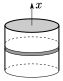
\includegraphics{drum}\qquad\qquad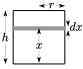
\includegraphics{drumX}
\end{center}
\end{efig}

\soln We are going to tackle this problem by applying the standard
integral calculus ``slice into small pieces'' strategy. This is how we computed areas and
volumes --- slice the problem into small pieces, work out how much each piece contributes,
and then add up the contributions using an integral.

\begin{itemize}
 \item Start by slicing the reservoir (or rather the fluid inside it) into thin,
horizontal, cylindrical pancakes, as in the figure above. We proceed by determining how
much work is required to pump out this pancake volume of fluid\footnote{Potential for a
bad ``work out how much work out'' pun here.}.
\item Each pancake is a squat cylinder with thickness $\dee{x}$ and circular cross
section of radius $r$ and area $\pi r^2$. Hence it has volume $\pi r^2 \dee{x}$ and mass
$\rho \times \pi r^2\dee{x}$.
\item Near the surface of the Earth gravity exerts a downward force of
$mg$ on a body of mass $m$. The constant $g=9.8$m/$\mathrm{sec}^2$
is called the \emph{standard acceleration due to gravity}\footnote{This quantity is not
actually constant --- it varies slightly across the surface of earth depending on local
density, height above sea-level and centrifugal force from the earth's rotation. It
is, for example, slightly higher in Oslo and slightly lower in Singapore. It is
actually \emph{defined} to be $9.80665$ m/$\mathrm{sec}^2$ by the International
Organisation for Standardization.}. For us to raise the pancake we have to apply a
compensating upward force of $mg$, which, for our pancake, is
\begin{align*}
  F &= g \rho \times \pi r^2\dee{x}
\end{align*}
\item To remove the pancake at height $x$ from the reservoir we need to
raise it to height $h$. So we have to lift it a distance $h-x$ using the force $F=\pi \rho
g r^2\dee{x}$, which takes work $ \pi\rho g r^2\,(h-x)\, \dee{x}$.

\item The total work to empty the whole reservoir is
\begin{align*}
W&= \int_0^h \pi\,\rho g\,r^2 (h-x)\dee{x}
= \pi\,\rho g\,r^2 \int_0^h  (h-x)\dee{x} \\
&=\pi\,\rho g\,r^2  \Big[hx -\frac{x^2}{2}\Big]_0^h \\
&=\frac{\pi}{2}\,\rho g\, r^2 h^2
\end{align*}
\item If we measure lengths in metres and mass in kilograms, then this
quantity has units of Joules. If we instead used feet and pounds\footnote{%
%Beware that the name ``pound'' is used for two \emph{different} units ---
%pound--force and pound--mass. The ``pound'' in foot--pound is pound--force.
It is extremely mysterious to the authors why a person would do science
or engineering in imperial units. One of the authors still has nightmares
about having had to do so as a student.} then this would
have units of ``foot--pounds''. One foot-pound is equal to
1.355817\dots Joules.
\end{itemize}

\end{eg}




\begin{eg}[Escape Velocity]\label{eg:WKgravity}
Suppose that you shoot a probe straight up from the surface of the Earth --- at what
initial speed must the probe move in order to escape Earth's gravity?

\soln We determine this by computing how much work must be done in order to escape
Earth's gravity. If we assume that all of this work comes from the probe's initial
kinetic energy, then we can establish the minimum initial velocity required.

\begin{itemize}
 \item
The work done by gravity when a mass moves from the surface of
the Earth to a height $h$ above the surface is
\begin{align*}
  W &= \int_0^h F(x) \dee{x}
\end{align*}
where $F(x)$ is the gravitational force acting on the mass at height $x$ above the
Earth's surface.

\item The gravitational force\footnote{Newton published his inverse square law of
universal gravitation in his Principia in 1687. His law states that the
gravitational force between two masses $m_1$ and $m_2$ is
\begin{align*}
  F &= -G \frac{m_1 m_2}{r^2}
\end{align*}
where $r$ is the distance separating the (centres of the) masses and $G=
6.674\times 10^{-11} \mathrm{N}\mathrm{m}^2/\mathrm{kg}^2$ is the gravitational constant.
Notice that $r$ measures the separation between the centres of the masses not the
distance between the surfaces of the objects.

Also, do not confuse $G$ with $g$ --- standard acceleration due to gravity. The first
measurement of $G$ was performed by Henry Cavendish in 1798 --- the interested reader
should look up the ``Cavendish experiment'' for details of this very impressive work.} of
the Earth acting on a particle of mass $m$ at a height $x$ above the surface of the Earth
is
\begin{align*}
F=-\frac{GMm}{(R+x)^2},
\end{align*}
where $G$ is the gravitational constant, $M$ is the mass of the Earth and
$R$ is the radius of the Earth. Note that $R+x$ is the distance from the object to
the centre of the Earth. Additionally, note that this force is negative because
gravity acts downward.

\item So the work done by gravity on the probe, as it travels from the surface of the
Earth to a height $h$, is
\begin{align*}
W&=-\int_0^h \frac{GMm}{(R+x)^2}\dee{x}\\
&=-GMm\int_0^h \frac{1}{(R+x)^2}\dee{x}
\intertext{A quick application of the substitution rule with $u=R+x$ gives}
&=-GMm \int_{u(0)}^{u(h)} \frac{1}{u^2} \dee{u}\\
&= -GMm \left[ -\frac{1}{u} \right]_{u=R}^{u=R+h} \\
&= \frac{GMm}{R+h} - \frac{GMm}{R}
\end{align*}
% We can find the indefinite integral of $\frac{1}{(R+x)^2}$
% by making the substitution $u=R+x$ and then integrating $\frac{1}{u^2}$.
% But we don't have to --- we already know, from Corollary ????,
% that
% \begin{align*}
% \int (ax+b)^n\,\dee{x} =\frac{(ax+b)^{n+1}}{a(n+1)}+C
% \end{align*}
% (check this by verifying that the derivative of the right hand
% side is $(ax+b)^n$)
% so that, choosing $a=1$, $b=R$ and $n=-2$,
% \begin{align*}
% \int \frac{1}{(R+x)^2}\ \dee{x} = -\frac{1}{R+x} + C
% \implies
% W=  \frac{GMm}{R+x}\bigg|_0^h
%   =\frac{GMm}{R+h} - \frac{GMm}{R}
% \end{align*}

\item So if the probe completely escapes the Earth and
travels all the way to $h=\infty$, gravity does work
\begin{align*}
\lim_{h\rightarrow\infty}\Big[\frac{GMm}{R+h} - \frac{GMm}{R}\Big]
=- \frac{GMm}{R}
\end{align*}
The minus sign means that gravity has removed energy $\frac{GMm}{R}$
from the probe.
\item To finish the problem we need one more assumption. Let us assume that all of this
energy comes from the probe's initial kinetic energy and that the probe is not
fitted with any sort of rocket engine. Hence the initial kinetic energy $\frac{1}{2}mv^2$
(coming from an initial velocity $v$) must be at least as large as the work computed
above. That is we need
\begin{align*}
\frac{1}{2}mv^2 &\ge \frac{GMm}{R} & \text{which rearranges to give}\\
v &\ge \sqrt{\frac{2GM}{R}}
\end{align*}
\item The right hand side of this inequality, $\sqrt{\frac{2GM}{R}}$, is called the
escape velocity.
\end{itemize}
\end{eg}

\begin{eg}[Lifting a Cable]\label{eg:WKcable}
A $10$--metre--long cable of mass $5$kg is used to lift a bucket of water,
with mass 8kg, out of a well. Find the work done.

\soln
Denote by $y$ the height of the bucket above the top of the water in the well.
So the bucket is raised from $y=0$ to $y=10$. The cable has mass density
$0.5$kg/m. So when the bucket is at height $y$,
\begin{itemize}\itemsep1pt \parskip0pt \parsep0pt %\itemindent-15pt
\item the cable that remains to be lifted has mass $0.5(10-y)$ kg and
\item the remaining cable and water is subject to a downward gravitational
force of magnitude $\big[0.5(10-y) + 8\big]g=\big[13-\frac{y}{2}\big]g$,
where $g=9.8$ m/sec$^2$.
\end{itemize}
So to raise the bucket from height $y$ to height $y+\dee{y}$ we need
to apply a compensating upward force of $\big[13-\frac{y}{2}\big]g$
through distance $\dee{y}$. This takes work
$\big[13-\frac{y}{2}\big]g\ \dee{y}$.
So the total work required is
\begin{equation*}
\int_0^{10}\Big[13-\frac{y}{2}\Big]g\ \dee{y}
=g\left[13 y-\frac{y^2}{4}\right]_0^{10}
=\big[130-25\big]g
=105 g
=1029\ \mathrm{J}
\end{equation*}

\end{eg}


\section{Averages}\label{sec avg}
\newcommand{\ave}{\mathrm{ave}}
\newcommand{\llt}{\left<}
\newcommand{\rgt}{\right>}

Another frequent\footnote{Awful pun. The two main approaches to statistics are
frequentism and Bayesianism; the latter named after Bayes' Theorem which is, in turn,
named for Reverend Thomas Bayes. While this (both the approaches to statistics
and their history and naming) is a very interesting and quite
philosophical topic, it is beyond the scope of this course. The interested reader has
plenty of interesting reading here to interest them.} application of integration is
computing averages and other statistical quantities. We will not spend too much time on
this topic --- that is best left to a proper course in statistics --- however, we will
demonstrate the application of integration to the problem of computing averages.

Let us start with the definition\footnote{
We are being a little loose here with the distinction between mean and average. To be
much more pedantic --- the average is the arithmetic mean. Other interesting ``means'' are
the geometric and harmonic means:
\begin{align*}
  \text{arithmetic mean} &= \frac{1}{n}\left( y_1 + y_2 + \cdots + y_n \right)\\
  \text{geometric mean} &= \left( y_1 \cdot y_2 \cdots y_n \right)^{\nicefrac{1}{n}}\\
  \text{harmonic mean} &= \left[\frac{1}{n}\left(
  \frac{1}{y_1} + \frac{1}{y_2} + \cdots \frac{1}{y_n}
  \right)\right]^{-1}
\end{align*}
All of these quantities, along with the median and mode, are ways to measure the typical
value of a set of numbers. They all have advantages and disadvantages --- another
interesting topic beyond the scope of this course, but plenty of fodder for the
interested reader and their favourite search engine. But let us put pedantry (and
beyond-the-scope-of-the-course-reading) aside and just use the terms average and mean
interchangeably for our purposes here.} of the average of a finite set of numbers.
\begin{defn}\label{def avg}
 The average (mean) of a set of $n$ numbers $y_1$, $y_2$, $\cdots$, $y_n$ is
\begin{align*}
y_\ave =\bar y = \llt y\rgt =\frac{y_1+y_2+\cdots+y_n}{n}
\end{align*}
The notations $y_\ave$, $\bar y$ and $\llt y\rgt$ are all commonly used
to represent the average.
\end{defn}

Now suppose that we want to take the average of a function $f(x)$ with $x$ running
continuously from $a$ to $b$. How do we even define what that means? A natural approach is
to
\begin{itemize}
\item select, for each natural number $n$, a sample of $n$, more or
less uniformly distributed, values of $x$ between $a$ and $b$,
\item take the average of the values of $f$ at the selected points,
\item and then take the limit as $n$ tends to infinity.
\end{itemize}
Unsurprisingly, this process looks very much like how we computed areas and volumes
previously. So let's get to it.
\begin{itemize}
\item
First fix any natural number $n$.
\item
Subdivide the interval $a\le x\le b$ into $n$ equal subintervals,
each of width $\De x=\frac{b-a}{n}$.
\item
The subinterval number $i$ runs from $x_{i-1}$ to $x_i$ with
$x_i=a+i\frac{b-a}{n}$.
\item
Select, for each $1\le i\le n$, one value of $x$
from subinterval number $i$ and call it $x_i^*$.
So $x_{i-1}\le x_i^*\le x_i$.
\item
The average value of $f$ at the selected points is
\begin{align*}
\frac{1}{n}\sum_{i=1}^n f(x_i^*)
=&\frac{1}{b-a}\sum_{i=1}^n f(x_i^*) \De x
&\text{since $\De x=\frac{b-a}{n}$}
\end{align*}
giving us a Riemann sum.
\end{itemize}
Now when we take the limit $n\rightarrow\infty$
we get exactly $\frac{1}{b-a}\int_a^b f(x)\dee{x}$. That's why we define
\begin{defn}\label{def:AVaverage}
Let $f(x)$ be an integrable function defined on the interval
$a\le x\le b$. The average value of $f$ on that interval is
\begin{align*}
f_\ave=\bar f=\llt f\rgt
=\frac{1}{b-a}\int_a^b f(x)\ \dee{x}
\end{align*}
\end{defn}

Consider the case when $f(x)$ is positive. Then rewriting Definition~\ref{def:AVaverage}
as
\begin{align*}
f_\ave\ (b-a) &= \int_a^b f(x)\dee{x} &
\raisebox{-0.5\height}{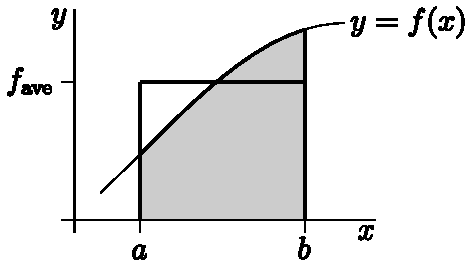
\includegraphics{areaAve}}
\end{align*}
gives us a link between the average value and the area under the curve. The right-hand
side is the area of the region
\begin{align*}
\big\{(x,y)\ \big|\ a\le x\le b,\ 0\le y\le f(x)\ \big\}
\end{align*}
while the left-hand side can be seen as the area of a rectangle of width $b-a$
and height $f_\ave$. Since these areas must be the same, we interpret $f_\ave$ as
the height of the rectangle which has the same width and the same area as
$\big\{(x,y)\ \big|\ a\le x\le b,\ 0\le y\le f(x)\ \big\}$.


Let us start with a couple of simple examples and then work our way up to harder ones.
\begin{eg}
 Let $f(x)= x$ and $g(x)=x^2$ and compute their average values
over $1 \leq x\leq 5$.

\soln We can just plug things into the definition.
\begin{align*}
  f_\ave &= \frac{1}{5-1}\int_1^5 x \dee{x} \\
  &= \frac{1}{4} \bigg[ \frac{x^2}{2} \bigg]_1^5 \\
  &= \frac{1}{8} (25-1) = \frac{24}{8} \\
  &= 3
\end{align*}
as we might expect. And then
\begin{align*}
g_\ave &= \frac{1}{5-1}\int_1^5 x^2 \dee{x} \\
  &= \frac{1}{4} \bigg[ \frac{x^3}{3} \bigg]_1^5 \\
  &= \frac{1}{12} (125-1) = \frac{124}{12} \\
&= \frac{31}{3}
\end{align*}
\end{eg}
Something a little more trigonometric
\begin{eg}
 Find the average value of $\sin(x)$ over $0 \leq x \leq \nicefrac{\pi}{2}$.

\soln Again, we just need the definition.
\begin{align*}
  \text{average} &= \frac{1}{\nicefrac{\pi}{2} - 0}
\int_0^{\nicefrac{\pi}{2}} \sin(x) \dee{x} \\
&= \frac{2}{\pi} \cdot \bigg[ -\cos(x) \bigg]_0^{\nicefrac{\pi}{2}} \\
&= \frac{2}{\pi} (-\cos(\nicefrac{\pi}{2})+\cos(0)) \\
&= \frac{2}{\pi}.
\end{align*}
\end{eg}

We could keep going\dots But better to do some more substantial examples.
\begin{eg}[Average velocity]\label{eg:AVvelocity}
Let $x(t)$ be the position at time $t$ of a car moving along the $x$--axis.
The velocity of the car at time $t$ is the derivative $v(t)=x'(t)$.
The average velocity of the car over the time interval $a\le t\le b$ is
\begin{align*}
v_\ave &= \frac{1}{b-a}\int_a^b v(t)\dee{t}\\
&=\frac{1}{b-a}\int_a^b x'(t)\dee{t}\\
&=\frac{x(b)-x(a)}{b-a} & \text{by the fundamental theorem of calculus.}
\end{align*}
The numerator in this formula is just the displacement (net distance travelled --- if
$x'(t)\ge 0$, it's the distance travelled) between time $a$ and time $b$ and the
denominator is just the time it took.

Notice that this is exactly the formula we used way back at the start of your
\emph{differential} calculus class to help introduce the idea of the derivative. Of
course this is a very circuitous way to get to this formula --- but it is reassuring that
we get the same answer.
\end{eg}

A very physics example.
\begin{eg}[Peak vs RMS voltage]
\label{eg:peakvsrms}When you plug a light bulb into a socket\footnote{A normal household socket delivers
alternating current, rather than the direct current USB supplies. At the risk of yet
another ``the interested reader'' suggestion --- the how and why household plugs supply
AC current is another worthwhile and interesting digression from studying integration.
The interested reader should look up the ``War of Currents''. The diligent and
interested reader should bookmark this, finish the section and come back to it later.}
and turn it on, it is subjected to a voltage
\begin{align*}
 V(t) &= V_0\sin(\omega t-\delta)
\end{align*}
where
\begin{itemize}
\item $V_0=170$ volts,
\item $\omega=2\pi\times 60$ (which corresponds to $60$ cycles per second\footnote{Some
countries supply power at 50 cycles per second. Japan actually supplies both --- 50
cycles in the east of the country and 60 in the west.})
and
\item the constant $\delta$ is an (unimportant) phase. It just shifts the time
at which the voltage is zero
\end{itemize}
The voltage $V_0$ is the ``peak voltage'' --- the maximum value the voltage takes over
time. More typically we quote the ``root mean square'' voltage\footnote{This example was
written in North America where the standard voltage supplied to homes is 120 volts. Most
of the rest of the world supplies homes with 240 volts. The main reason for this
difference is the development of the light bulb. The USA electrified earlier when the best
voltage for bulb technology was 110 volts. As time went on, bulb technology improved and
countries that electrified later took advantage of this (and the cheaper transmission
costs that come with higher voltage) and standardised at 240 volts. So many digressions in
this section!}  (or RMS-voltage). In this example we explain the difference, but to
simplify the calculations, let us simplify the voltage function and just use
\begin{align*}
  V(t) &= V_0 \sin(t)
\end{align*}

Since the voltage is a sine-function, it takes both positive and negative values. If we
take its simple average over 1 period then we get
\begin{align*}
  V_\ave &= \frac{1}{2\pi-0} \int_0^{2\pi} V_0 \sin(t) \dee{t}\\
  &= \frac{V_0}{2\pi}\bigg[ - \cos(t)\bigg]_0^{2\pi} \\
  &= \frac{V_0}{2\pi}\left( -\cos(2\pi) + \cos 0\right) = \frac{V_0}{2\pi}(-1+1)\\
  &= 0
\end{align*}
This is clearly not a good indication of the typical voltage.

What we actually want here is a measure of how far the voltage is from zero. Now we could
do this by taking the average of $|V(t)|$, but this is a little harder to work with.
Instead we take the average of the square\footnote{For a finite
set of numbers one can compute the ``quadratic mean'' which is another way to generalise
the notion of the average:
\begin{align*}
  \text{quadratic mean}
&= \sqrt{\frac{1}{n}\left(y_1^2 + y_2^2 + \cdots + y_n^2 \right) }
\end{align*}
} of the voltage (so it is always positive) and then take the square root at the
end. That is
\begin{align*}
  V_\mathrm{rms}
  &= \sqrt{\frac{1}{2\pi-0} \int_0^{2\pi} V(t)^2 \dee{t}}\\
  &= \sqrt{\frac{1}{2\pi} \int_0^{2\pi} V_0^2 \sin^2(t) \dee{t}}\\
  &= \sqrt{\frac{V_0^2}{2\pi} \int_0^{2\pi} \sin^2(t) \dee{t}}
\end{align*}
This is called the ``root mean square'' voltage.

Though we do know how to integrate sine and cosine, we don't (yet) know how to integrate
their squares. A quick look at double-angle formulas\footnote{A quick glance at
Appendix~\ref{sec must deriv} will refresh your memory.} gives us a way to eliminate the
square:
\begin{align*}
  \cos(2\theta) =1-2\sin^2\theta \implies \sin^2\theta=\frac{1-\cos(2\theta)}{2}
\end{align*}
Using this we manipulate our integrand a little more:
\begin{align*}
V_\mathrm{rms} &= \sqrt{\frac{V_0^2}{2\pi} \int_0^{2\pi}
\frac{1}{2}(1-\cos(2t)) \dee{t}}\\
&= \sqrt{
\frac{V_0^2}{4\pi}
\bigg[t - \frac{1}{2}\sin(2t)  \bigg]_0^{2\pi}
}\\
&= \sqrt{
\frac{V_0^2}{4\pi} \left(2\pi - \frac{1}{2}\sin(4\pi) - 0 + \frac{1}{2}\sin(0) \right)
}\\
&= \sqrt{
\frac{V_0^2}{4\pi} \cdot 2\pi
}\\
&= \frac{V_0}{\sqrt{2}}
\end{align*}
So if the peak voltage is 170 volts then the RMS voltage is $\frac{170}{\sqrt{2}}\approx
120.2$.
\end{eg}


Continuing this very physics example:
\begin{eg}\label{eg:AVpower}
Let us take our same light bulb with voltage (after it is plugged in) given by
\begin{align*}
 V(t) &= V_0\sin(\omega t-\delta)
\end{align*}
where
\begin{itemize}
\item $V_0$ is the peak voltage,
\item $\omega=2\pi\times 60$, and
\item the constant $\delta$ is an (unimportant) phase.
\end{itemize}
If the light bulb is ``100 watts'', then what is its resistance?

To answer this question we need the following facts from physics.
\begin{itemize}
\item
If the light bulb has resistance $R$ ohms, this causes, by Ohm's law, a current of
\begin{align*}
      I(t) &= \frac{1}{R} V(t) &
\end{align*}
(amps) to flow through the light bulb.
\item
The current $I$ is the number of units of charge moving through the bulb per unit time.
\item
The voltage is the energy required to move one unit of charge through the bulb.
\item
The power is the energy used by the bulb per unit time and is measured in watts.
\end{itemize}
So the power is the product of the current times the voltage and, so
\begin{equation*}
P(t)=I(t)V(t)
=\frac{V(t)^2}{R}
=\frac{V_0^2}{R}\sin^2(\omega t-\delta)
\end{equation*}
The average power used over the time interval $a\le t\le b$ is
\begin{align*}
P_\ave &= \frac{1}{b-a}\int_a^b P(t)\ \dee{t}
        = \frac{V_0^2}{R(b-a)}\int_a^b \sin^2(\omega t-\delta)\ \dee{t}
\end{align*}
Notice that this is almost exactly the form we had in the previous example when computing
the root mean square voltage.


Again we simplify the integrand using the identity
\begin{equation*}
\cos(2\theta) =1-2\sin^2\theta
\implies \sin^2\theta=\frac{1-\cos(2\theta)}{2}
\end{equation*}
So
\begin{align*}
P_\ave &= \frac{1}{b-a}\int_a^b P(t)\ \dee{t}
  = \frac{V_0^2}{2R(b-a)}\int_a^b \big[1-\cos(2\omega t-2\delta)\big]\ \dee{t} \\[0.1in]
&=\frac{V_0^2}{2R(b-a)}\bigg[t-\frac{\sin(2\omega t-2\delta)}{2\omega}\bigg]_a^b \\[0.1in]
&=\frac{V_0^2}{2R(b-a)}\bigg[b-a-\frac{\sin(2\omega b-2\delta)}{2\omega}
  +\frac{\sin(2\omega a-2\delta)}{2\omega}\bigg]\\[0.1in]
&=\frac{V_0^2}{2R}
   -\frac{V_0^2}{4\omega R(b-a)}\big[\sin(2\omega b-2\delta)-\sin(2\omega a-2\delta)\big]
\end{align*}
In the limit as the length of the time interval $b-a$ tends to infinity,
this converges to $\frac{V_0^2}{2R}$. The resistance $R$ of a
``100 watt bulb''  obeys
\begin{align*}
\frac{V_0^2}{2R} &=100 & \text{so that} &&
R &= \frac{V_0^2}{200}.
\end{align*}
We finish this example off with two side remarks.
\begin{itemize}
  \item
  If we translate the peak voltage to the root mean square voltage using
\begin{align*}
  V_0 &= V_\mathrm{rms} \cdot \sqrt{2}
\end{align*}
then we have
\begin{align*}
  P &= \frac{V^2_{\mathrm{rms}}}{R}
\end{align*}
  \item If we were using direct voltage rather than alternating current then the
computation is
much simpler. The voltage and current are constants, so
\begin{align*}
  P &= V \cdot I & \text{but $I = V/R$ by Ohm's law} \\
  &= \frac{V^2}{R}
\end{align*}
So if we have a direct current giving voltage equal to the root mean square voltage, then
we would expend the same power.
\end{itemize}

\end{eg}

\subsection*{Optional --- Return to the Mean Value Theorem}
Here is another application of the Definition~\ref{def:AVaverage} of the average value of a function on an interval. The following theorem can be
thought of as an analogue of the mean value theorem (which was covered in your
differential calculus class) but for integrals. The theorem says that a continuous function 
$f(x)$ must be exactly equal to its average value for some $x$. For example, if you
went for a drive along the $x$--axis and you were at $x(a)$ at time $a$ and at $x(b)$ at
time $b$, then your velocity $x'(t)$ had to be exactly your average velocity
$\frac{x(b)-x(a)}{b-a}$ at some time $t$ between $a$ and $b$. In particular,
if your average velocity was greater than the speed limit, you were definitely
speeding at some point during the trip. This is, of course, no great 
surprise\footnote{There are many unsurprising things that are true, but there are also many
unsurprising things that surprisingly turn out to be false. Mathematicians like to
prove things - surprising or not.}.

\begin{theorem}[Mean Value Theorem for Integrals]\label{thm:AVmvt}
Let $f(x)$ be a continuous function on the interval $a\le x\le b$.
Then there is some $c$ obeying $a < c < b$ such that
\begin{align*}
\frac{1}{b-a}\int_a^b f(x)\,\dee{x}=f(c) \qquad\text{or}\qquad
\int_a^b f(x)\dee{x} = f(c)\,(b-a)
\end{align*}
\end{theorem}

\begin{proof}
We will apply the mean value theorem (Theorem~\eref{CLP1}{thm:DIFFmvt} in the CLP-1 text) to
the function
\begin{equation*}
F(x) = \int_a^x f(t)\,\dee{t}
\end{equation*}
By the part 1 of the fundamental theorem of calculus 
(Theorem~\ref{thm:INTfundthmofcalc}),
$F'(x)=f(x)$, so the mean value theorem says that there is a $a<c<b$ with
\begin{align*}
f(c) &= F'(c) = \frac{F(b)-F(a)}{b-a}
=\frac{1}{b-a}\left\{\int_a^b f(t)\,\dee{t}-\int_a^a f(t)\,\dee{t}\right\}
\\
&=\frac{1}{b-a}\int_a^b f(x)\,\dee{x}
\end{align*}
\end{proof}

In the next section, we will encounter an application in which we want to take the average value of a function $f(x)$, but in doing so we want some values 
of $x$ to count more than other values of $x$. That is, we want to weight 
some $x$'s more than other $x$'s. To do so, we choose a ``weight function'' 
$w(x)\ge 0$ with $w(x)$ larger for more important $x$'s.  Then we define the weighted average of $f$ as follows.
\begin{defn}\label{def:Wtaverage}
Let $f(x)$ and $w(x)$ be integrable functions defined on the interval
$a\le x\le b$ with $w(x)\ge 0$ for all $a\le x\le b$ and with $\int_a^b w(x)\, \dee{x}>0$.  The average value of $f$ on that interval, weighted by $w$, is
\begin{align*}
\frac{\int_a^b f(x)\,w(x)\,\dee{x}}{\int_a^b w(x)\,\dee{x}}
\end{align*}
We typically refer to this simply as the weighted average of $f$.
\end{defn}\noindent
Here are a few remarks concerning this definition.
\begin{itemize}
\item
The definition has been rigged so that, if $f(x)=1$ for all $x$, then the 
weighted average of $f$ is $1$, no matter what weight function $w(x)$ is used.
\item
If the weight function $w(x)=C$ for some constant $C>0$ then the weighted average
\begin{equation*}
\frac{\int_a^b f(x)\,w(x)\,\dee{x}}{\int_a^b w(x)\,\dee{x}}
=\frac{\int_a^b f(x)\,C\,\dee{x}}{\int_a^b C\,\dee{x}}
=\frac{\int_a^b f(x)\,\dee{x}}{b-a}
\end{equation*}
is just the usual average.
\item
For any function $w(x)\ge 0$ and any $a<b$, we have $\int_a^b w(x)\, \dee{x}\ge 0$.
But for the definition of weighted average to make sense, we need to be able to divide
by $\int_a^b w(x)\, \dee{x}$. So we need $\int_a^b w(x)\, \dee{x}\ne 0$. 

\end{itemize}

The next theorem says that a continuous function $f(x)$ must be equal to
its weighted average at some point $x$.
\begin{theorem}[Mean Value Theorem for Weighted Integrals]\label{thm:AVwtmvt}
Let $f(x)$ and $w(x)$ be continuous functions on the interval $a\le x\le b$.
Assume that $w(x)>0$ for all $a<x<b$. Then there is some $c$ 
obeying $a < c < b$ such that
\begin{align*}
\frac{\int_a^b f(x)\,w(x)\,\dee{x}}{\int_a^b w(x)\,\dee{x}}=f(c) \qquad\text{or}\qquad
\int_a^b f(x)\,w(x)\,\dee{x} = f(c)\int_a^b w(x)\,\dee{x}
\end{align*}
\end{theorem}

\begin{proof}
We will apply the generalised mean value theorem (Theorem~\eref{CLP1}{thm:GMVT} in the CLP-1 text) to
\begin{equation*}
F(x) = \int_a^x f(t)\,w(t)\dee{t}\qquad
G(x) = \int_a^x w(t)\dee{t}
\end{equation*}
By the part 1 of the fundamental theorem of calculus 
(Theorem~\ref{thm:INTfundthmofcalc}),
$F'(x)=f(x)w(x)$ and $G'(x)=w(x)$, so the generalised mean value theorem 
says that there is a $a<c<b$ with
\begin{align*}
f(c) &= \frac{F'(c)}{G'(c)} = \frac{F(b)-F(a)}{G(b)-G(a)}
=\frac{\int_a^b f(t)\,w(t)\dee{t}-\int_a^a f(t)w(t)\,\dee{t}}
  {\int_a^b w(t)\dee{t}-\int_a^a w(t)\dee{t}}
\\
&=\frac{\int_a^b f(t)\,w(t)\,\dee{t}}{\int_a^b w(t)\,\dee{t}}
\end{align*}
\end{proof}

\begin{eg}\label{eg:weightedAverage}
In this example, we will take a number of weighted averages of the simple function 
$f(x)=x$ over the simple interval $a=1\le x\le 2=b$. As $x$ increases from $1$ to $2$,
the function $f(x)$ increases linearly from $1$ to $2$. So it is no shock that the 
ordinary average of $f$ is exactly its middle value:
\begin{equation*}
\frac{1}{b-a}\int_a^b f(t)\,\dee{t}
=\frac{1}{2-1}\int_1^2 t\,\dee{t}
=\frac{3}{2}
\end{equation*}  
Pick any natural number $N\ge 1$ and consider the weight function $w_N(x)=x^N$. Note that
$w_N(x)$ increases as $x$ increases. So $w_N(x)$ weights bigger $x$'s more than it weights 
smaller $x$'s. In particular $w_N$ weights the point $x=2$ by a factor of $2^N$
(which is greater than $1$ and grows to infinity as $N$ grows to infinity) more than it weights the point $x=1$. The weighted average of $f$ is
\begin{align*}
\frac{\int_a^b f(t)\,w_N(t)\,\dee{t}}{\int_a^b w_N(t)\,\dee{t}}
&=\frac{\int_1^2 t^{N+1}\,\dee{t}}{\int_1^2 t^N\,\dee{t}}
=\frac{\frac{2^{N+2}-1}{N+2}}{\frac{2^{N+1}-1}{N+1}}
=\frac{N+1}{N+2}\ \frac{2^{N+2}-1}{2^{N+1}-1} \\
&=\begin{cases}
   \frac{2\times 7}{3\times 3}  = 1.555  &\text{if }N=1 \\[0.05in]
   \frac{3\times 15}{4\times 7} = 1.607  &\text{if }N=2 \\[0.05in]
   \frac{4\times 31}{5\times 15}= 1.653  &\text{if }N=3 \\[0.05in]
   \frac{5\times 63}{6\times 31}= 1.694  &\text{if }N=4 
%   \\ 1.802  &\text{if }N=8  
   \\ 1.889  &\text{if }N=16  
%   \\ 1.941  &\text{if }N=32  
%   \\ 1.970  &\text{if }N=64  
%   \\ 1.985  &\text{if }N=128  
   \\ 1.992  &\text{if }N=256  
   \end{cases}
\end{align*}
As we would expect, the $w_N$-weighted average is between $1.5$ (which is the ordinary, unweighted, average) and $2$ (which is the biggest value of $f$ in the interval) and 
grows as $N$ grows. The limit as $N\rightarrow\infty$ of the $w_N$-weighted average is
\begin{align*}
\lim_{N\rightarrow\infty}\frac{N+1}{N+2}\ \frac{2^{N+2}-1}{2^{N+1}-1} 
&=\lim_{N\rightarrow\infty}\frac{N+2-1}{N+2}\ \frac{2^{N+2}-2+1}{2^{N+1}-1} \\
&=\lim_{N\rightarrow\infty}\left[1-\frac{1}{N+2}\right]\ 
                           \left[2+\frac{1}{2^{N+1}-1}\right] \\
&=2
\end{align*} 

\end{eg}

\begin{eg}\label{eg:needPositive}
Here is an example which shows what can go wrong with Theorem~\ref{thm:AVwtmvt}
if we allow the weight function $w(x)$ to change sign. Let $a=-0.99$ and
$b=1$. Let
\begin{align*}
w(x)&=\begin{cases}1&\text{if $x\ge 0$}\\
                  -1&\text{if $x<0$} \end{cases} 
\\
f(x)&=\begin{cases}x&\text{if $x\ge 0$}\\
                  0&\text{if $x<0$} \end{cases} 
\end{align*} 
Then
\begin{align*}
\int_a^b f(x)\,w(x)\,\dee{x} &= \int_0^1 x\,\dee{x} =\frac{1}{2} 
\\ 
\int_a^b w(x)\,\dee{x} &= \int_0^1 \dee{x} -\int_{-0.99}^0\dee{x}
                        = 1 - 0.99
                        = 0.01
\end{align*}
As $c$ runs from $a$ to $b$, $f(c)\int_a^b w(x)\,\dee{x}=0.01 f(c)$ runs from 
$0$ to $0.01$ and, in particular, never takes a value anywhere near 
$\int_a^b f(x)\,w(x)\,\dee{x}=\frac{1}{2}$. There is no $c$ value which works.
\end{eg}



\section{Centre of Mass and Torque}\label{sec com}
\subsection{Centre of Mass}
If you support a body at its center of mass (in a uniform gravitational
field) it balances perfectly. That's the definition of the center of mass
of the body.%
\vadjust{
\begin{efig}
\begin{center}
    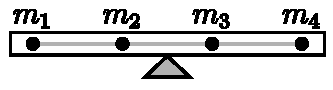
\includegraphics{seesaw3}
\end{center}
\end{efig}
}
If the body consists of a finite number of masses $m_1$, $\cdots$, $m_n$
attached to an infinitely strong, weightless (idealized) rod with mass
number $i$ attached at position $x_i$, then the center of mass is
at the (weighted) average value of $x$:
\begin{equation}\label{eq:weightedrod}
\bar x =\frac{\sum_{i=1}^n m_ix_i}{\sum_{i=1}^n m_i}
\end{equation}
The denominator $m=\sum_{i=1}^n m_i$ is the total mass of the body.
%The numerator
%\begin{equation*}
%\mu=\sum_{i=1}^n m_ix_i
%\end{equation*}
%is called the moment of the body about the origin.
This formula for the
center of mass is derived in the following (optional) section. See
\eqref{eq:TRQfulcrum}.


For many (but certainly not all) purposes an (extended rigid) body acts like
a point particle located at its center of mass. For example it is very
common to treat the Earth as a point particle. Here is a more detailed
example in which we think of a body as being made up of a number of component
parts and compute the center of mass of the body as a whole by using the
center of masses of the component parts. Suppose that we have a dumbbell
which consists of
\begin{itemize}\itemsep1pt \parskip0pt \parsep0pt %\itemindent-15pt
\item a left end made up of particles of masses $m_{l,1}$, $\cdots$, $m_{l,3}$
located at $x_{l,1}$, $\cdots$, $x_{l,3}$ and
\item a right end made up of particles of masses $m_{r,1}$, $\cdots$, $m_{r,4}$
located at $x_{r,1}$, $\cdots$, $x_{r,4}$ and
\item an infinitely strong, weightless (idealized) rod joining all of the
particles.
\end{itemize}
Then the mass and center of mass of the left end are
\begin{equation*}
M_l=m_{l,1}+\cdots +m_{l,3}\qquad
\bar X_l = \frac{m_{l,1}x_{l,1}+\cdots +m_{l,3}x_{l,3}}{M_l}
\end{equation*}
and the mass and center of mass of the right end are
\begin{equation*}
M_r=m_{r,1}+\cdots +m_{r,4}\qquad
\bar X_r = \frac{m_{r,1}x_{r,1}+\cdots +m_{r,4}x_{r,4}}{M_r}
\end{equation*}
The mass and center of mass of the entire dumbbell are
\begin{align*}
M&= m_{l,1}+\cdots +m_{l,3}\  +\  m_{r,1}+\cdots +m_{r,4} \\
 &= M_l+M_r \\
\bar x &=\frac{m_{l,1}x_{l,1}+\cdots +m_{l,3}x_{l,3}\ +\
              m_{r,1}x_{r,1}+\cdots +m_{r,4}x_{r,4}}{M} \\
       &=\frac{M_l \bar X_l + M_r \bar X_r}{M_r+M_l}
\end{align*}
So we can compute the center of mass of the entire dumbbell by treating
it as being made up of two point particles, one of mass $M_l$ located at
the centre of mass of the left end, and one of mass $M_r$ located at the
center of mass of the right end.

\begin{eg}[Work and Centre of Mass]\label{eg:TRQcomWork}
Here is another example in which an extended body acts like a point particle located at its centre of mass. Imagine that there are a finite number of
masses $m_1,\cdots,m_n$ arrayed along a (vertical) $z$--axis with mass
number $i$ attached at height $z_i$. Note  that the total mass of the array
is $M=\sum_{i=1}^n m_i$ and that the centre of mass of the array is at height
\begin{align*}
\bar z =\frac{\sum_{i=1}^n m_iz_i}{\sum_{i=1}^n m_i}
       =\frac{1}{M} \sum_{i=1}^n m_iz_i
\end{align*}
Now suppose that we lift all of the masses, against gravity, to height $Z$.
So after the lift there is a total mass $M$ located at height $Z$.
The $i^{\rm th}$ mass is subject to a downward gravitational force of $m_i g$.
So to lift the $i^{\rm th}$ mass we need to apply a compensating
upward force of $m_ig$ through a distance of $Z-z_i$. This takes work
$m_i g (Z-z_i)$. So the total  work required to lift all $n$ masses is
\begin{align*}
\text{Work} &= \sum_{i=1}^n  m_i g (Z-z_i) \\
            &= g Z \sum_{i=1}^n  m_i  -g \sum_{i=1}^n  m_i z_i \\
            &= g Z M - g M \bar z \\
            & =Mg(Z-\bar z)\hskip1.0in
\raisebox{-0.15\height}[5pt][15pt]{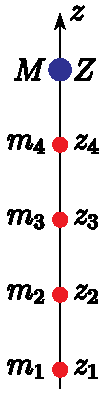
\includegraphics{array}}
\end{align*}
So the work required to lift the array of $n$ particles is identical
to the work required to lift a single particle, whose mass, $M$, is
the total mass of the array, from height $\bar z$, the centre of mass
of the array, to height $Z$.
\end{eg}


\begin{eg}[Example \ref{eg:TRQcomWork}, continued]\label{eg:TRQcomWorkB}
Imagine, as in Example \ref{eg:TRQcomWork}, that there are a finite number of
masses $m_1,\cdots,m_n$ arrayed along a (vertical) $z$--axis with mass
number $i$ attached at height $z_i$. Again, the total mass and centre of
mass of the array are
\begin{equation*}
M=\sum_{i=1}^n m_i \qquad
\bar z =\frac{\sum_{i=1}^n m_iz_i}{\sum_{i=1}^n m_i}
       =\frac{1}{M} \sum_{i=1}^n m_iz_i
\end{equation*}
Now suppose that we lift, for each $1\le i\le n$, mass number $i$,
against gravity, from its initial height $z_i$ to a final height $Z_i$.
So after the lift we have a new array of masses with total mass and
centre of  mass
\begin{equation*}
M=\sum_{i=1}^n m_i \qquad
\bar Z =\frac{\sum_{i=1}^n m_iZ_i}{\sum_{i=1}^n m_i}
       =\frac{1}{M} \sum_{i=1}^n m_iZ_i
\end{equation*}
To lift the $i^{\rm th}$ mass took work $m_i g (Z_i-z_i)$. So the total
work required to lift all $n$ masses was
\begin{align*}
\text{Work} &= \sum_{i=1}^n  m_i g (Z_i-z_i) \\
            &= g  \sum_{i=1}^n  m_i Z_i  -g \sum_{i=1}^n  m_i z_i \\
            &= g M \bar Z - g M \bar z =Mg(\bar Z-\bar z)
\end{align*}
So the work required to lift the array of $n$ particles  is identical
to the work required to lift a single particle, whose mass, $M$, is
the total mass of the array, from height $\bar z$, the initial centre of mass
of the array, to height $\bar Z$, the final centre of mass of the array.
\end{eg}


Now we'll extend the above ideas to cover more general classes of bodies.
If the body consists of mass distributed continuously along a straight
line, say with mass density $\rho(x)$kg/m and with $x$ running from $a$ to
$b$, rather than consisting of a finite number of point masses,
the formula for the center of mass becomes
\begin{equation}\label{eq:TRQvariabledensityrod}
\bar x = \frac{\int_a^b x\ \rho(x)\,\dee{x}}{\int_a^b \rho(x)\,\dee{x}}
\end{equation}
Think of $\rho(x)\,\dee{x}$ as the mass of the ``almost point particle''
between $x$ and $x+\dee{x}$.

If the body is a two dimensional object, like a metal plate, lying in
the $xy$--plane, its center of mass is a point $(\bar x,\bar y)$
with $\bar x$ being the (weighted) average value of the $x$--coordinate
over the body and $\bar y$ being the (weighted) average value of the
$y$--coordinate over the body. To be concrete, suppose the body fills the
region
\begin{equation*}
\big\{\ (x,y)\ \big|\ a\le x\le b,\ B(x)\le y\le T(x)\ \big\}
\end{equation*}
in the $xy$--plane. For simplicity, we will assume that the density
of the body is a constant, say $\rho$. When the density is constant,
the center of mass is also called the \emph{centroid} and is thought of
as the geometric center of the body.

To find the centroid of the body, we use our standard ``slicing''
strategy. We slice the body into thin vertical strips, as illustrated in
the figure below.%
\vadjust{
\begin{efig}
\begin{center}
   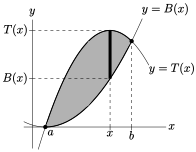
\includegraphics{centroidGen}
\end{center}
\end{efig}
}
Here is a detailed description of a generic strip.
\begin{itemize}\itemsep1pt \parskip0pt \parsep0pt %\itemindent-15pt
\item The strip has width $\dee{x}$.
\item Each point of the strip has essentially the same $x$--coordinate.
Call it $x$.
\item The top of the strip is at $y=T(x)$ and the bottom of the strip is
at $y=B(x)$.
\item So the strip has
\begin{itemize}\itemsep1pt \parskip0pt \parsep0pt %\itemindent-15pt
\item height $T(x)-B(x)$
\item area $[T(x)-B(x)]\,\dee{x}$
\item mass $\rho[T(x)-B(x)]\,\dee{x}$
\item centroid, i.e. middle point, $\big(x\,,\,\frac{B(x)+T(x)}{2}\big)$.
\end{itemize}
\end{itemize}
In computing the centroid of the entire body, we may treat each strip as
a single particle of mass $\rho[T(x)-B(x)]\,\dee{x}$ located at
$\big(x\,,\,\frac{B(x)+T(x)}{2}\big)$. So the mass of the entire body is
\begin{subequations}\label{eq:TRQcentroid}
\begin{alignat}{4}
M&= \rho\int_a^b [T(x)-B(x)]\,\dee{x} =\rho A\hidewidth \\
\intertext{where $A=\int_a^b [T(x)-B(x)]\,\dee{x}$ is the area of the region.
The coordinates of the centroid are}
\bar x %&= \frac{\int_a^b x \,dm}{M}
        &= \frac{\int_a^b x\ \overbrace{\rho[T(x)-B(x)]\,\dee{x}}
                     ^{\mathrm{mass\ of\ slice}}}
                {M }
        &&= \frac{\int_a^b x [T(x)-B(x)]\,\dee{x}}{A} \\
\bar y %&= \frac{\int_a^b \frac{B(x)+T(x)}{2} \,dm}{M }\
       &= \frac{\int_a^b\!\!\!\!\overbrace{\tfrac{B(x)+T(x)}{2}}
                     ^{\mathrm{average}\ y\ \mathrm{on\ slice}}\!\!
                 \overbrace{\rho[T(x)-B(x)]\,\dee{x}}
                     ^{\mathrm{mass\ of\ slice}}}
          {M }\
       &&= \frac{\int_a^b\, [T(x)^2-B(x)^2]\,\dee{x}}{2A}
\end{alignat}
\end{subequations}
We can of course also slice up the body using horizontal slices.%
\vadjust{
\begin{efig}
\begin{center}
   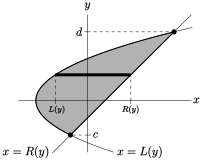
\includegraphics{centroidY}
\end{center}
\end{efig}
}
If the body has constant density $\rho$ and fills the region
\begin{equation*}
\big\{\ (x,y)\ \big|\ L(y)\le x\le R(y),\ c\le y\le d\ \big\}
\end{equation*}
then the same computation as above gives the mass of the body to be
\begin{subequations}\label{eq:TRQcentroidy}
\begin{alignat}{4}
M&= \rho\int_c^d [R(y)-L(y)]\,\dee{y} =\rho A\hidewidth \\
\intertext{where $A=\int_c^d [R(y)-L(y)]\,\dee{y}$ is the area of the region,
and gives the coordinates of the centroid to be}
\bar x %&= \frac{\int_c^d \frac{R(y)+L(y)}{2} \,dm}{M }\
       &= \frac{\int_c^d\!\!\!\!\overbrace{\tfrac{R(y)+L(y)}{2}}
                            ^{\mathrm{average}\ x\ \mathrm{on\ slice}}\!\!
                         \overbrace{\rho[R(y)-L(y)]\,\dee{y}}
                             ^{\mathrm{mass\ of\ slice}}}
                             {M } \
       &&= \frac{\int_c^d\, [R(y)^2-L(y)^2]\,\dee{y}}{2A} \\
\bar y %&= \frac{\int_c^d y \,dm}{M}
       &= \frac{\int_c^d y\ \overbrace{\rho[R(y)-L(y)]\,\dee{y}}
                               ^{\mathrm{mass\ of\ slice}}}
                                   {M }
       &&= \frac{\int_c^d y [R(y)-L(y)]\,\dee{y}}{A}
\end{alignat}
\end{subequations}


\begin{eg}\label{eq:TRQcentroidA}
 Find the $x$--coordinate of the centroid (centre of gravity)
of the plane region $R$ that lies in the first quadrant $x\ge 0, \ y\ge
0$ and inside the ellipse $4x^2+9y^2=36$. (The area bounded by the ellipse
$\frac{x^2}{a^2}+\frac{y^2}{b^2}=1$ is $\pi ab$ square units.)

\begin{efig}
\begin{center}
    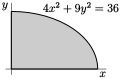
\includegraphics{centroidQuarterEllipse}
\end{center}
\end{efig}

\soln In standard form $4x^2+9y^2=36$ is $\frac{x^2}{9}+\frac{y^2}{4}=1$.
So, on $R$, $x$ runs from $0$ to $3$ and $R$ has area
$A=\frac{1}{4}\pi\times 3\times 2=\frac{3}{2}\pi$. For each fixed $x$,
between $0$ and $3$, $y$ runs from $0$ to $2\sqrt{1-\frac{x^2}{9}}$.
So, applying (\ref{eq:TRQcentroid}.b) with $a=0$, $b=3$,
$T(x)=2\sqrt{1-\frac{x^2}{9}}$ and $B(x)=0$,
\begin{equation*}
\bar x =\frac{1}{A}\int_0^3 x\,T(x)\,\dee{x}
=\frac{1}{A}\int_0^3 x\,2\sqrt{1-\frac{x^2}{9}}\,\dee{x}
=\frac{4}{3\pi}\int_0^3 x\sqrt{1-\frac{x^2}{9}}\,\dee{x}
\end{equation*}
Sub in $u=1-\frac{x^2}{9}$, $\dee{u}=-\frac{2}{9}x\,\dee{x}$.
\begin{equation*}
\bar x
=-\frac{9}{2}\frac{4}{3\pi}\int_1^0 \sqrt{u}\,\dee{u}
=-\frac{9}{2}\frac{4}{3\pi}\Big[\frac{u^{3/2}}{3/2}\Big]_1^0
=-\frac{9}{2}\frac{4}{3\pi}\Big[-\frac{2}{3}\Big]
=\frac{4}{
\pi}
\end{equation*}
\end{eg}

\goodbreak
\begin{eg}\label{eg:TRQcentroidBa}
  Find the centroid of the quarter circular disk $x\ge 0$,
$y\ge 0$, $x^2+y^2\le r^2$.

\begin{efig}
\begin{center}
    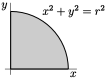
\includegraphics{centroidQuarterCircle}
\end{center}
\end{efig}

\soln  By symmetry, $\bar x=\bar y$. The area of the quarter disk
is $A=\frac{1}{4}\pi r^2$. By (\ref{eq:TRQcentroid}.b) with $a=0$, $b=r$,
$T(x)=\sqrt{r^2-x^2}$ and $B(x)=0$,
\begin{equation*}
\bar x = \frac{1}{A}\int_0^r x\sqrt{r^2-x^2}\,\dee{x}
\end{equation*}
To evaluate the integral, sub in $u=r^2-x^2$, $\dee{u}=-2x\,\dee{x}$.
\begin{equation}\label{eq:TRQcentroidB}
\int_0^r x\sqrt{r^2-x^2}\,\dee{x} = \int_{r^2}^0 \sqrt{u}\,\frac{\dee{u}}{-2}
= -\frac{1}{2}\Big[\frac{u^{3/2}}{3/2}\Big]^0_{r^2}
= \frac{r^3}{3}
\end{equation}
So
\begin{equation*}
\bar x
= \frac{4}{\pi r^2}\Big[\frac{r^3}{3}\Big]
=\frac{4r}{3\pi}
\end{equation*}

As we observed above, we should have $\bar x=\bar y$. But, just for practice,
let's compute $\bar y$ by the integral formula (\ref{eq:TRQcentroid}.c),
again with $a=0$, $b=r$, $T(x)=\sqrt{r^2-x^2}$ and $B(x)=0$,
\begin{alignat*}{3}
\bar y & =  \frac{1}{2A}\int_0^r \big(\sqrt{r^2-x^2}\big)^2\,\dee{x}\
 &&=  \frac{2}{\pi r^2}\int_0^r \big(r^2-x^2\big)\,\dee{x} \\
 &=  \frac{2}{\pi r^2}\Big[r^2x-\frac{x^3}{3}\Big]_0^r
 &&=  \frac{2}{\pi r^2}\frac{2r^3}{3} \\
 &=\frac{4r}{3\pi}
\end{alignat*}
as expected.
\end{eg}

\goodbreak
\begin{eg}\label{eg:TRQcentroidBaa}
  Find the centroid of the half circular disk $y\ge 0$, $x^2+y^2\le r^2$.

\begin{efig}
\begin{center}
    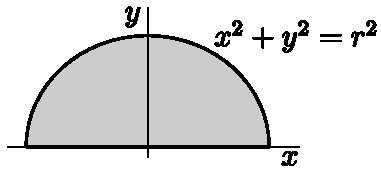
\includegraphics{centroidHalfCircle.pdf}
\end{center}
\end{efig}

\soln  Once again, we have a symmetry ---- namely the half disk is symmetric about the $y$--axis. So the centroid lies on the $y$--axis and $\bar x=0$.
The area of the half disk is $A=\frac{1}{2}\pi r^2$.
By (\ref{eq:TRQcentroid}.c), with $a=-r$, $b=r$, $T(x)=\sqrt{r^2-x^2}$ and $B(x)=0$,
\begin{alignat*}{3}
\bar y & =  \frac{1}{2A}\int_{-r}^r \big(\sqrt{r^2-x^2}\big)^2\,\dee{x}\
 &&=  \frac{1}{\pi r^2}\int_{-r}^r \big(r^2-x^2\big)\,\dee{x} \\
 &=  \frac{2}{\pi r^2}\int_0^r \big(r^2-x^2\big)\,\dee{x}
\qquad\text{since the integrand is even}\hidewidth\\
 &=  \frac{2}{\pi r^2}\Big[r^2x-\frac{x^3}{3}\Big]_0^r  \\
 &=\frac{4r}{3\pi}
\end{alignat*}
\end{eg}


\goodbreak
\begin{eg}\label{eg:TRQcentroidBb}
 Find the centroid of the region $R$ in the diagram.

\begin{efig}
\begin{center}
    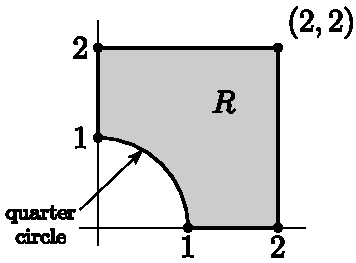
\includegraphics{PSIVc}
\end{center}
\end{efig}


\soln
By symmetry, $\bar x=\bar y$. The region $R$
is a $2\times 2$ square with one quarter of a circle of radius $1$ removed
and so has area $2\times 2-\frac{1}{4}\pi=\frac{16-\pi}{4}$.
The top of $R$ is $y=T(x)=2$. The bottom is $y=B(x)$ with
$B(x)\!=\!\sqrt{1-x^2}$ when $0\le x\le 1$ and $B(x)\!=\!0$
when $1\le x\le 2$. So
\begin{align*}
\bar y = \bar x &=\frac{1}{A}\bigg[\int_0^1x[2-\sqrt{1-x^2}]\,\dee{x}
              +\int_1^2x[2-0]\,\dee{x}\bigg]\cr
&=\frac{4}{16-\pi}\bigg[x^2\big|_0^1
            +x^2\big|_1^2-\int_0^1x\sqrt{1-x^2}\,\dee{x}\bigg]\\
&=\frac{4}{16-\pi}\Big[4-\frac{1}{3}\Big]
       \qquad\qquad\text{by \eqref{eq:TRQcentroidB} with $r=1$}\\
&=\frac{44}{48-3\pi}
\end{align*}
\end{eg}
\goodbreak

\begin{eg}\label{eg:TRQcentroidC}
Prove that the centroid of any triangle
is located at the point of intersection of the medians.
A median of a triangle is a line segment joining a vertex
to the midpoint of the opposite side.

\begin{efig}
\begin{center}
    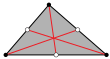
\includegraphics{medianA}
\end{center}
\end{efig}


\soln Choose a coordinate system so that the vertices of the triangle
are located at $(a,0)$, $(0,b)$ and $(c,0)$. (In the figure below,
$a$ is negative.)%
\vadjust{
\begin{efig}
\begin{center}
    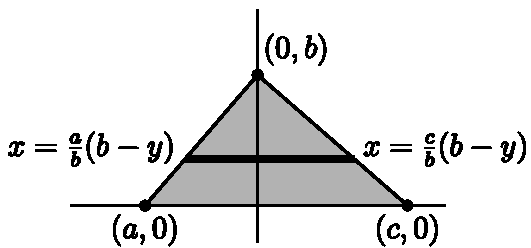
\includegraphics{median}
\end{center}
\end{efig}}
The line joining $(a,0)$ and $(0,b)$ has equation $bx+ay=ab$.
(Check that $(a,0)$ and $(0,b)$ both really are on this line.)
The line joining $(c,0)$ and $(0,b)$ has equation $bx+cy=bc$.
(Check that $(c,0)$ and $(0,b)$ both really are on this line.)
Hence for each fixed $y$ between $0$ and $b$, $x$ runs from
$a-\frac{a}{b}y$ to $c-\frac{c}{b}y$.


We'll use horizontal strips to compute $\bar x$ and $\bar y$. We could
just apply \eqref{eq:TRQcentroidy} with $c=0$, $d=b$,
$R(y)= \frac{c}{b}(b-y)$ (which is gotten by solving $bx+cy=bc$ for $x$) and
$L(y)= \frac{a}{b}(b-y)$ (which is gotten by solving $bx+ay=ab$ for $x$).

But rather than memorizing or looking up those formulae,
we'll derive them for this example.
So consider a thin strip at height $y$ as illustrated in the figure above.
\begin{itemize}\itemsep1pt \parskip0pt \parsep0pt %\itemindent-15pt
\item
The strip has length
\begin{equation*}
\ell(y)=\Big[\frac{c}{b}(b-y)-\frac{a}{b}(b-y)\Big]=\frac{c-a}{b}(b-y)
\end{equation*}
\item The strip has width $\dee{y}$.
\item
On this strip, $y$ has average value $y$.
\item
On this strip, $x$ has average value
$\frac{1}{2}\big[\frac{a}{b}(b-y)+\frac{c}{b}(b-y)\big]=\frac{a+c}{2b}(b-y)$.
\end{itemize}
As the area of the triangle is
$A=\half (c-a)b$,
\begin{align*}
\bar y&=\frac{1}{A}\int_0^b y\ \ell(y)\ \dee{y}
=\frac{2}{(c-a)b}\int_0^b y\frac{c-a}{b}(b-y)\ \dee{y}
=\frac{2}{b^2}\int_0^b (by-y^2)\ \dee{y}
=\frac{2}{b^2}\Big(b\frac{b^2}{2}-\frac{b^3}{3}\Big)
\\
&=\frac{2}{b^2}\frac{b^3}{6}=\frac{b}{3}\displaybreak[0]\\[0.1in]
\bar x&=\frac{1}{A}\int_0^b \frac{a+c}{2b}(b-y)\ \ell(y)\ \dee{y}
=\frac{2}{(c-a)b}\int_0^b \frac{a+c}{2b}(b-y)\frac{c-a}{b}(b-y)\ \dee{y}
=\frac{a+c}{b^3}\int_0^b (y-b)^2\ \dee{y}
\\
&=\frac{a+c}{b^3}\Big[\frac{1}{3}(y-b)^3\Big]_0^b
=\frac{a+c}{b^3}\ \frac{b^3}{3}
=\frac{a+c}{3}
\end{align*}
We have found that the centroid of the triangle is at
$(\bar x,\bar y)=\big(\frac{a+c}{3},\frac{b}{3}\big)$. We
shall now show that this point lies on all three medians.
\begin{itemize}\itemsep1pt \parskip0pt \parsep0pt %\itemindent-15pt
\item One vertex is at $(a,0)$. The opposite side runs from
$(0,b)$ and $(c,0)$ and so has midpoint $\half(c,b)$. The line
from $(a,0)$ to $\half(c,b)$ has slope $\frac{b/2}{c/2-a}=\frac{b}{c-2a}$
and so has equation $y=\frac{b}{c-2a}(x-a)$. As
$\frac{b}{c-2a}(\bar x-a)
=\frac{b}{c-2a}\big(\frac{a+c}{3}-a\big)
=\frac{1}{3}\frac{b}{c-2a}(c+a-3a)
=\frac{b}{3}
=\bar y$, the centroid does indeed lie on this median.
In this computation we have implicitly assumed that $c\ne 2a$ so that
the denominator $c-2a\ne 0$. In the event that $c=2a$, the median runs from
$(a,0)$ to $\big(a,\frac{b}{2}\big)$ and so has equation $x=a$. When
$c=2a$ we also have $\bar x=\frac{a+c}{3}=a$, so that the centroid still
lies on the median.

\item Another vertex is at $(c,0)$. The opposite side runs from
$(a,0)$ and $(0,b)$ and so has midpoint $\half(a,b)$. The line
from $(c,0)$ to $\half(a,b)$ has slope $\frac{b/2}{a/2-c}=\frac{b}{a-2c}$
and so has equation $y=\frac{b}{a-2c}(x-c)$. As
$\frac{b}{a-2c}(\bar x-c)
=\frac{b}{a-2c}\big(\frac{a+c}{3}-c\big)
=\frac{1}{3}\frac{b}{a-2c}(a+c-3c)
=\frac{b}{3}
=\bar y$, the centroid does indeed lie on this median.
In this computation we have implicitly assumed that $a\ne 2c$ so that
the denominator $a-2c\ne 0$. In the event that $a=2c$, the median runs from
$(c,0)$ to $\big(c,\frac{b}{2}\big)$ and so has equation $x=c$. When
$a=2c$ we also have $\bar x=\frac{a+c}{3}=c$, so that the centroid still
lies on the median.


\item The third vertex is at $(0,b)$. The opposite side runs from
$(a,0)$ and $(c,0)$ and so has midpoint $\big(\frac{a+c}{2},0\big)$.
The line from $(0,b)$ to $\big(\frac{a+c}{2},0\big)$ has slope
$\frac{-b}{(a+c)/2}=-\frac{2b}{a+c}$
and so has equation $y=b-\frac{2b}{a+c}x$. As
$b-\frac{2b}{a+c}\bar x
=b-\frac{2b}{a+c}\frac{a+c}{3}
=\frac{b}{3}
=\bar y$, the centroid does indeed lie on this median.
This time, we have implicitly assumed that $a+c\ne 0$.
In the event that $a+c=0$, the median runs from
$(0,b)$ to $(0,0)$ and so has equation $x=0$. When
$a+c=0$ we also have $\bar x=\frac{a+c}{3}=0$, so that the centroid still
lies on the median.
\end{itemize}


%The midpoint of the line joining $(0,b)$ and $(c,0)$ is $\half(c,b)$.
%The point two thirds of the way from $(a,0)$ to $\half(c,b)$ is
%$\frac{1}{3}(a,0)+\frac{2}{3}\half(c,b)
%=\big(\frac{a+c}{3},\frac{b}{3}\big)=(\bar x,\bar y)$
%as desired.
\end{eg}


\goodbreak
\subsection{Optional --- Torque}

Newton's law of motion says that the position $x(t)$
of a single particle moving under the influence
of a force $F$ obeys $mx''(t)=F$. Similarly, the positions $x_i(t)$,
$1\le i\le n$, of a set of particles moving under the influence
of forces $F_i$ obey $mx_i''(t)=F_i$, $1\le i\le n$. Often systems of
interest consist of some small number of rigid bodies. Suppose that
we are interested in the motion of a single rigid body, say a piece
of wood. The piece of wood is made up of a huge number of atoms.
So the system of equations determining the motion of all of the
individual atoms in the piece of wood is huge. On the other hand,
because the piece of wood is rigid, its configuration is completely
determined by the position of, for example, its centre of mass and
its orientation. (Rather than get into what is precisely meant by
``orientation'', let's just say that it is certainly determined by,
for example, the positions of a few of the corners of the piece of wood).
It is
possible to extract from the  huge system of equations that determine
the motion of all of the individual atoms, a small system of equations
that determine the motion of the centre of mass and the orientation.
We can avoid some vector analysis, that is beyond the scope of this
course, by assuming that our rigid body is moving in two rather than
three dimensions.

So, imagine a piece of wood moving in the $xy$--plane.%
\vadjust{
\begin{efig}
\begin{center}
    
\includegraphics{seesaw}
\end{center}
\end{efig}
}
Furthermore, imagine that the piece of wood consists of a huge number of
particles joined by a huge number of weightless but very strong steel rods.
The steel rod joining particle number one to particle number two just
represents a force acting between particles number one and two.
Suppose that
\begin{itemize}\itemsep1pt \parskip0pt \parsep0pt %\itemindent-15pt
\item there are $n$ particles, with particle number $i$ having
mass $m_i$
\item at time $t$, particle number $i$ has $x$--coordinate
$x_i(t)$ and $y$--coordinate $y_i(t)$
\item at time $t$,  the external force (gravity and the like)
acting on particle number $i$ has $x$--coordinate
$H_i(t)$ and $y$--coordinate $V_i(t)$. Here $H$ stands for horizontal and
$V$ stands for vertical.
\item at time $t$, the force acting on particle number $i$,
due to the steel rod joining particle number $i$ to particle number $j$
 has $x$--coordinate $H_{i,j}(t)$ and $y$--coordinate $V_{i,j}(t)$. If
there is no steel rod joining particles number $i$ and $j$, just set
$H_{i,j}(t)=V_{i,j}(t)=0$. In particular, $H_{i,i}(t)=V_{i,i}(t)=0$.
\end{itemize}
The only assumptions that we shall make about the steel rod forces
are
\begin{description}
\item[(A1)] for each $i\ne j$, $H_{i,j}(t)=-H_{j,i}(t)$ and
$V_{i,j}(t)=-V_{j,i}(t)$. In words, the steel rod joining particles $i$
and $j$ applies equal and opposite forces to particles $i$ and $j$.
\item[(A2)] for each $i\ne j$, there is a function $M_{i,j}(t)$ such
that $H_{i,j}(t)=M_{i,j}(t)\big[x_i(t)-x_j(t)\big]$ and
$V_{i,j}(t)=M_{i,j}(t)\big[y_i(t)-y_j(t)\big]$. In words, the force due
to the rod joining particles $i$ and $j$ acts parallel to the line
joining particles $i$ and $j$. For (A1) to be true, we need
$M_{i,j}(t)=M_{j,i}(t)$.
\end{description}

\noindent
Newton's law of motion, applied to particle number $i$,  now tells us that
%\refstepcounter{equation}\label{eq:TRQnewton}
%\begin{align}
%m_i x''_i(t)&= H_i(t)+\sum_{j=1}^n H_{i,j}(t)\tag{$\ref{eq:TRQnewton}.X_i$}\\
%m_i y''_i(t)&= V_i(t)+\sum_{j=1}^n V_{i,j}(t)\tag{$\ref{eq:TRQnewton}.Y_i$}
%\end{align}
\begin{align}
m_i x''_i(t)&= H_i(t)+\sum_{j=1}^n H_{i,j}(t)\tag{$X_i$}\\
m_i y''_i(t)&= V_i(t)+\sum_{j=1}^n V_{i,j}(t)\tag{$Y_i$}
\end{align}
Adding up all of the equations $(X_i)$, for
$i=1,\ 2,\ 3,\ \cdots,\ n$
and adding up all of the equations $(Y_i)$,
for $i=1,\ 2,\ 3,\ \cdots,\ n$ gives
\begin{align}
\sum_{i=1}^n m_i x''_i(t)&= \sum_{i=1}^n H_i(t)+\sum_{1\le i,j\le n} H_{i,j}(t)
      \tag{$\Sigma_iX_i$}\\
\sum_{i=1}^n m_i y''_i(t)&= \sum_{i=1}^n V_i(t)+\sum_{1\le i,j\le n} V_{i,j}(t)
      \tag{$\Sigma_iY_i$}
\end{align}
The sum $\sum_{1\le i,j\le n} H_{i,j}(t)$ contains $H_{1,2}(t)$
exactly once and it also contains $H_{2,1}(t)$ exactly once and these two
terms cancel exactly, by assumption (A1). In this way, all terms in
$\sum_{1\le i,j\le n} H_{i,j}(t)$
with $i\ne j$ exactly cancel. All terms with $i=j$ are assumed to be zero.
So $\sum_{1\le i,j\le n} H_{i,j}(t)=0$. Similarly,
$\sum_{1\le i,j\le n} V_{i,j}(t)=0$, so the equations $(\Sigma_iX_i)$
and $(\Sigma_iY_i)$ simplify to
\begin{align}
\sum_{i=1}^n m_i x''_i(t)&= \sum_{i=1}^n H_i(t)
              \tag{$\Sigma_iX_i$}\\
\sum_{i=1}^n m_i y''_i(t)&= \sum_{i=1}^n V_i(t)
     \tag{$\Sigma_iY_i$}
\end{align}
Denote by
\begin{equation*}
M=\sum\limits_{i=1}^n m_i
\end{equation*}
the total mass of the system, by \begin{equation*}
X(t)=\frac{1}{M}\sum\limits_{i=1}^n m_ix_i(t)\qquad \text{and}\qquad
Y(t)=\frac{1}{M}\sum\limits_{i=1}^n m_iy_i(t)
\end{equation*}
the $x$-- and $y$--coordinates of the centre of mass of the system
at time $t$ and by
\begin{equation*}
H(t)=\sum\limits_{i=1}^n H_i(t) \qquad\text{ and }\qquad
V(t)=\sum\limits_{i=1}^n V_i(t)
\end{equation*}
the $x$-- and $y$--coordinates of the total external force acting
on the system at time $t$. In this notation, the equations
$(\Sigma_iX_i)$ and $(\Sigma_iY_i)$ are
\begin{equation}\label{eq:TRQcofmeqn}
MX''(t)=H(t)\qquad MY''(t)=V(t)
\end{equation}
So the centre of mass of the system moves just like a single particle of
mass $M$ subject to the total external force.

Now multiply equation $(Y_i)$ by $x_i(t)$, subtract from it
equation $(X_i)$ multiplied by $y_i(t)$, and sum over $i$.
This gives the equation ${\sum_i\big[x_i(t)\,(Y_i)-y_i(t)\,(X_i)\big]}$:
\begin{equation*}
\sum_{i=1}^n m_i\big[x_i(t)y''_i(t)-y_i(t)x''_i(t)\big]
= \sum_{i=1}^n \big[x_i(t)V_i(t)-y_i(t)H_i(t)\big]
+\sum_{1\le i,j\le n} \big[x_i(t)V_{i,j}(t)-y_i(t)H_{i,j}(t)\big]
\end{equation*}
By the assumption (A2)
\begin{align*}
x_1(t)V_{1,2}(t)-y_1(t)H_{1,2}(t)
&=x_1(t)M_{1,2}(t)\big[y_1(t)-y_2(t)\big]
-y_1(t)M_{1,2}(t)\big[x_1(t)-x_2(t)\big]\\
&=M_{1,2}(t)\big[y_1(t)x_2(t)-x_1(t)y_2(t)\big]\\
%%%
x_2(t)V_{2,1}(t)-y_2(t)H_{2,1}(t)
&=x_2(t)M_{2,1}(t)\big[y_2(t)-y_1(t)\big]
-y_2(t)M_{2,1}(t)\big[x_2(t)-x_1(t)\big]\\
&=M_{2,1}(t)\big[-y_1(t)x_2(t)+x_1(t)y_2(t)\big]\\
&=M_{1,2}(t)\big[-y_1(t)x_2(t)+x_1(t)y_2(t)\big]
\end{align*}
So the $i=1$, $j=2$ term in $\sum_{1\le i,j\le n}
\big[x_i(t)V_{i,j}(t)-y_i(t)H_{i,j}(t)\big]$
exactly cancels the $i=2$, $j=1$ term.
In this way all of the terms in $\sum_{1\le i,j\le n}
\big[x_i(t)V_{i,j}(t)-y_i(t)H_{i,j}(t)\big]$
with $i\ne j$ cancel. Each term with $i=j$ is exactly zero.
So $\sum_{1\le i,j\le n} \big[x_i(t)V_{i,j}(t)-y_i(t)H_{i,j}(t)\big]=0$
and
\begin{equation*}
\sum_{i=1}^n m_i\big[x_i(t)y''_i(t)-y_i(t)x''_i(t)\big]
= \sum_{i=1}^n \big[x_i(t)V_i(t)-y_i(t)H_i(t)\big]
\end{equation*}
Define
\begin{align*}
L(t)&= \sum_{i=1}^n m_i\big[x_i(t)y'_i(t)-y_i(t)x'_i(t)\big]\\
T(t)&=\sum_{i=1}^n \big[x_i(t)V_i(t)-y_i(t)H_i(t)\big]
\end{align*}
In this notation
\begin{equation}\label{eq:TRQrotmoteqn}
\frac{d\hfill}{dt}L(t)=T(t)
\end{equation}
\begin{itemize}
\item Equation \eqref{eq:TRQrotmoteqn} plays the role of Newton's law of
motion for rotational motion.
\item $T(t)$ is called the torque and plays the role of ``rotational force''.
\item
$L(t)$ is called the angular momentum (about the origin) and is a measure
of the rate at which the piece of wood  is rotating.
\begin{itemize}
\item
For example, if a particle of mass $m$ is traveling in a
circle of radius $r$, centred on the origin, at $\omega$ radians per unit time,
then $x(t)=r\cos(\omega t)$,  $y(t)=r\sin(\omega t)$ and
\begin{align*}
m\big[x(t)y'(t)-y(t)x'(t)\big]
&= m \big[r\cos(\omega t)\ r\omega\cos(\omega t)
       -r\sin(\omega t)\ \big(-r\omega\sin(\omega t)\big)\big] \\
&=m r^2\ \omega
\end{align*}
is proportional to $\omega$, which is the rate of rotation about the origin.
\begin{efig}
\begin{center}
    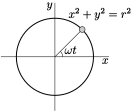
\includegraphics{circularMotion}
\end{center}
\end{efig}
\end{itemize}
\end{itemize}
In any event, in order for the piece of wood to remain stationary,
that is to have $x_i(t)$ and $y_i(t)$ be constant for all
$1\le i\le n$, we need to have
\begin{equation*}
X''(y)=Y''(t)=L(t)=0
\end{equation*}
and then
equations \eqref{eq:TRQcofmeqn} and \eqref{eq:TRQrotmoteqn} force
\begin{equation*}
H(t)=V(t)=T(t)=0
\end{equation*}

Now suppose that the piece of wood is a seesaw that is long and thin and
is lying on the $x$--axis, supported on a fulcrum at $x=p$.
Then every $y_i=0$ and the torque simplifies to
$T(t)=\sum_{i=1}^n x_i(t)V_i(t)$. The forces consist of
\begin{itemize}
\item
gravity, $m_ig$, acting downwards on particle number $i$, for each
$1\le i\le n$ and the%
\item
force $F$ imposed by the fulcrum that is pushing straight up on the particle
at $x=p$.
\begin{efig}
\begin{center}
    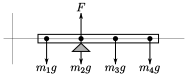
\includegraphics{seesaw2}
\end{center}
\end{efig}
\end{itemize}
So
\begin{itemize}
\item
The net vertical force is $V(t)=F-\sum\limits_{i=1}^n m_ig
=F-Mg$. If the seesaw is to remain stationary, this must be zero so that
$F=Mg$.
\item
The total torque (about the origin) is
\begin{equation*}
T=Fp-\sum_{i=1}^n m_ig x_i
=Mgp-\sum_{i=1}^n m_ig x_i
%=\sum_{i=1}^n m_igp-\sum_{i=1}^n m_ig x_i
%=\sum_{i=1}^n m_ig (p-x_i)
\end{equation*}
If the seesaw is to remain stationary, this must also be zero and the fulcrum
must be placed at
\begin{equation}\label{eq:TRQfulcrum}
p=\frac{1}{M}\sum_{i=1}^n m_i x_i
\end{equation}
which is the centre of mass of the piece of wood.
\end{itemize}


% \longsection{Coming soon --- Separable differential equations}{Coming soon ---
% Separable DEs}\label{sec sep de}


\section{Separable Differential Equations}\label{sec sep de}


A differential equation is an equation for an unknown function that
involves the derivative of the unknown function. Differential equations
play a central role in modelling a huge number of different phenomena.
Here is a table giving a bunch of named differential equations and what
they are used for. It is far from complete.

\begin{center}
\renewcommand{\arraystretch}{1.4}
     \begin{tabular}{|c|c|}
        \hline
  Newton's Law of Motion
      & describes motion of particles \\ \hline
  Maxwell's equations
      &describes electromagnetic radiation \\ \hline
  Navier--Stokes equations
      &describes fluid motion \\ \hline
  Heat equation
      &describes heat flow \\ \hline
  Wave equation
      &describes wave motion \\ \hline
  Schr\"odinger equation
      &describes atoms, molecules and crystals \\ \hline
  Stress-strain equations
      &describes elastic materials \\ \hline
  Black--Scholes models
      &used for pricing financial options \\ \hline
  Predator--prey equations
      &describes ecosystem populations  \\ \hline
  Einstein's equations
      &connects gravity and geometry  \\ \hline
  Ludwig--Jones--Holling's equation
      &models spruce budworm/Balsam fir ecosystem  \\ \hline
  Zeeman's model
      &models heart beats and nerve impulses \\ \hline
  Sherman--Rinzel--Keizer model
      &for electrical activity in Pancreatic $\beta$--cells  \\ \hline
  Hodgkin--Huxley equations
      &models nerve action potentials  \\
  \hline
     \end{tabular}
\renewcommand{\arraystretch}{1.0}
\end{center}

We are just going to scratch the surface of the study of differential
equations. Most universities offer half a dozen different undergraduate
courses on various aspects of differential equations. We will just look
at one special, but important, type of equation.

\subsection{Separate and Integrate}

\begin{defn}\label{def:SDEsepdiffeq}
A \emph{separable differential equation} is an equation for a function
$y(x)$ of the form
\begin{equation*}
\diff{y}{x}(x) = f(x)\ g\big(y(x)\big)
\end{equation*}
\end{defn}

We'll start by developing a recipe for solving separable differential
equations. Then we'll look at many examples.
Usually one suppresses the argument of $y(x)$  and writes the
equation\footnote{Look at the right hand side of the equation.
The $x$--dependence is separated from the $y$--dependence. That's
the reason for the name ``separable''.}
\begin{equation*}
\diff{y}{x} = f(x)\ g(y)
\end{equation*}
and solves such an equation by cross multiplying/dividing
to get all of the $y$'s, including the $\dee{y}$ on one side of
the equation and all of the $x$'s, including the $\dee{x}$, on the
other side of the equation.
\begin{equation*}
\frac{\dee{y}}{g(y)}=f(x)\,\dee{x}
\end{equation*}
(We are of course assuming that $g(y)$ is nonzero.)
Then you integrate both sides
\begin{equation}\label{eq:SDEbasicSln}
\int\frac{\dee{y}}{g(y)}=\int f(x)\,\dee{x}
\end{equation}
This looks illegal, and indeed is illegal --- $\diff{y}{x}$ is not a fraction.
But we'll now see that the answer is still correct. This procedure is simply
a mnemonic device to help you remember the answer \eqref{eq:SDEbasicSln}.
\begin{itemize}
\item
Our goal is to find all functions $y(x)$ that obey
$
\diff{y}{x}(x) = f(x)\ g\big(y(x)\big)
$.
\item
Assuming that $g$ is nonzero,
\begin{align*}
y'(x) = f(x)\ g(y(x))
&\iff \frac{y'(x)}{g(y(x))}=f(x)
\iff \int\frac{y'(x)}{g(y(x))}\,\dee{x}= \int f(x)\,\dee{x} \\
&\iff \int\frac{\dee{y}}{g(y)}\bigg|_{y=y(x)}= \int f(x)\,\dee{x} \\
&\qquad \text{with the substitution $y=y(x)$, $\dee y = y'(x)\,\dee{x}$}
\end{align*}
\item
That's our answer \eqref{eq:SDEbasicSln} again.
\end{itemize}

% Let $G(y)$ be an
%antiderivative of $\frac{1}{g(y)}$ (i.e. $G'(y)=\frac{1}{g(y)}$) and
%$F(x)$ be an antiderivative of $f(x)$ (i.e. $F'(x)=f(x))$.
%If we reinstate the argument of $y$, \eqref{eq:SDEbasicSln} is
%\begin{equation}\label{eq:SDEbasicSlnRig}
%G\big(y(x)\big) = F(x) + C
%\end{equation}
%To check that a function $y(x)$ obeys
%$\diff{y}{x}(x) = f(x)\ g\big(y(x)\big)$ if and only if it obeys
%\eqref{eq:SDEbasicSlnRig}, just differentiate both sides of
%\eqref{eq:SDEbasicSlnRig} with respect to $x$. By the chain rule
%\begin{align*}
%G\big(y(x)\big) = F(x) + C
%&\iff G'\big(y(x)\big)\ y'(x) = F'(x)
%\iff \frac{y'(x)}{g(y(x))}=f(x) \\
%&\iff y'(x) = f(x)\ g(y(x))
%\end{align*}
%(We have again assumed that $g(y)$ is nonzero.)

Let $G(y)$ be an antiderivative of $\frac{1}{g(y)}$
(i.e. $G'(y)=\frac{1}{g(y)}$) and $F(x)$ be an antiderivative of $f(x)$
(i.e. $F'(x)=f(x)$). If we reinstate the argument of $y$, 
\eqref{eq:SDEbasicSln} is
\begin{equation}\label{eq:SDEbasicSlnRig}
G\big(y(x)\big) = F(x) + C
\end{equation}
Observe that the solution \eqref{eq:SDEbasicSlnRig} contains an arbitrary
constant, $C$. The value of this arbitrary constant \emph{can not}
be determined by the differential equation. You need additional data
to determine it. Often this data consists of the value of the unknown
function for one value of $x$. That is, often the problem you have to solve
is of the form
\begin{equation*}
\diff{y}{x}(x) = f(x)\ g\big(y(x)\big)\qquad y(x_0)=y_0
\end{equation*}
where $f(x)$ and $g(y)$ are given functions and $x_0$ and $y_0$ are
given numbers. This type of problem is called an ``initial value problem''.
It is solved by first using the method above to find the general solution
to the differential equation, including the arbitrary constant $C$,
and then using the ``initial condition'' $y(x_0)=y_0$ to determine the
value of $C$. We'll see examples of this shortly.

\begin{eg}\label{eg:SDEsdeAA}
The differential equation
\begin{equation*}
\diff{y}{x} = xe^{-y}
\end{equation*}
is separable, and we now find all of its solutions by using our mnemonic
device. We start by cross--multiplying so as to move all $y$'s to the left
hand side and all $x$'s to the right hand side.
\begin{equation*}
e^y\,\dee{y} = x\,\dee{x}
\end{equation*}
Then we integrate both sides
\begin{equation*}
\int e^y\dee{y} = \int x\dee{x}
\iff e^y = \frac{x^2}{2}+C
\end{equation*}
The $C$ on the right hand side contains both the arbitrary constant
for the indefinite integral $\int e^y\dee{y}$ and the arbitrary constant for
the indefinite integral  $\int x\dee{x}$. Finally, we solve for $y$,
which is really a function of $x$.
\begin{equation*}
y(x) = \log\Big(\frac{x^2}{2}+C\Big)
\end{equation*}
Recall that we are using $\log$ to refer to the natural (base $e$)
logarithm.

Note that $C$ is an arbitrary constant. It can take any value. It cannot be
determined by the differential equation itself. In applications $C$ is usually
determined by a requirement that $y$ take some prescribed value (determined by the  application) when $x$ is some prescribed value. For example, suppose that we wish to find a function $y(x)$ that obeys both
\begin{equation*}
\diff{y}{x} = xe^{-y}\qquad\text{and}\qquad y(0)=1
\end{equation*}
We know that, to have $\diff{y}{x} = xe^{-y}$ satisfied, we must have
$y(x) = \log\big(\frac{x^2}{2}+C\big)$, for some constant $C$. To also have
$y(0)=1$, we must have
\begin{align*}
1=y(0)=\log\Big(\frac{x^2}{2}+C\Big)\bigg|_{x=0}=\log C
\iff \log C =1
\iff C=e
\end{align*}
So our final solution is $y(x) = \log\big(\frac{x^2}{2}+e\big)$.
\end{eg}



\begin{eg}\label{eg:SDEsdeFrist}
Let $a$ and $b$ be any two constants. We'll now solve the family of differential
equations
\begin{equation*}
\diff{y}{x} =a(y-b)
\end{equation*}
using our mnemonic device.
\begin{align*}
\frac{\dee{y}}{y-b} =a\,\dee{x}
&\implies
\int \frac{\dee{y}}{y-b}= \int a\,\dee{x}
\implies
\log|y-b|= ax+c
\implies
|y-b|= e^{ax+c} =e^c e^{ax} \\
&\implies y-b = C e^{ax}
\end{align*}
where $C$ is either $+e^c$ or $-e^c$. Note that as $c$ runs over
all real numbers, $+e^c$ runs over all strictly positive real
numbers and $-e^c$ runs over all strictly negative real numbers.
So, so far, $C$ can be any real number except $0$.
But we were a bit sloppy here. We implicitly
assumed that $y-b$ was nonzero, so that we could divide it across.
None--the--less, the constant function $y=b$, which corresponds
to $C=0$, is a perfectly good solution --- when $y$
is the constant function $y=b$, both $\diff{y}{x}$ and $a(y-b)$ are zero.
So the general solution to $\diff{y}{x} =a(y-b)$ is $y(x)=C e^{ax}+b$, where
the constant $C$ can be any real number. Note that when $y(x)=C e^{ax}+b$
we have $y(0)=C+b$. So $C=y(0)-b$ and the general solution is
\begin{equation*}
y(x) = \{y(0)-b\}\,e^{ax} + b
\end{equation*}

\end{eg}

This is worth stating as a theorem.
\begin{theorem}\label{thm:linearODE}
Let $a$ and $b$ be constants.
The differentiable function $y(x$) obeys the differential equation
\begin{equation*}
\diff{y}{x} =a(y-b)
\end{equation*}
if and only if
\begin{equation*}
y(x) = \{y(0)-b\}\,e^{ax} + b
\end{equation*}
\end{theorem}

\begin{eg}\label{eg:SDEsdeA}
 Solve $\diff{y}{x}=y^2$

\soln When $y\ne 0$,
\begin{equation*}
\diff{y}{x}=y^2
\implies \frac{\dee{y}}{y^2}=\dee{x}
\implies \frac{y^{-1}}{-1}=x+C
\implies y=-\frac{1}{x+C}
\end{equation*}
When $y=0$, this computation breaks down because  $ \frac{\dee{y}}{y^2}$
contains a division by 0. We can check if the function $y(x)=0$
satisfies the differential equation by just subbing it in:
\begin{equation*}
y(x)=0\implies y'(x)=0,\ y(x)^2=0\implies y'(x)=y(x)^2
\end{equation*}
So $y(x)=0$ is a solution and the full solution is
\begin{equation*}
y(x)=0 \text{ or } y(x)=-\frac{1}{x+C}, \text{ for any constant $C$}
\end{equation*}
\end{eg}

\begin{eg}\label{eg:SDEraindrop}
When a raindrop falls it increases
in size so that its mass $m(t)$, is a function of time $t$. The rate of
growth of mass, i.e. $\frac{dm}{dt}$, is $km(t)$ for some positive
constant $k$. According to Newton's law of motion, $\diff{}{t} (mv)=gm$,
where $v$ is the velocity of the raindrop (with $v$ being positive for
downward motion) and $g$ is the acceleration due to gravity. Find the
terminal velocity, $\lim\limits_{t\rightarrow\infty}v(t)$, of a raindrop.

\soln In this problem we have two unknown functions, $m(t)$ and $v(t)$,
and two differential equations, $\frac{dm}{dt}=km$ and $\diff{}{t} (mv)=gm$.
The first differential equation, $\frac{dm}{dt}=km$, involves only
$m(t)$, not $v(t)$, so we use it to determine $m(t)$.
By Theorem \ref{thm:linearODE}, with $b=0$, $a=k$, $y$ replaced
by $m$ and $x$ replaced by $t$,
\begin{equation*}
\diff{m}{t}=km
%\implies \frac{dm}{m}=k\,\dee{t}
%\implies \log m=kt+c\implies m=de^{kt}\hbox{ where }d=e^c
\implies m(t) = m(0) e^{kt}
\end{equation*}
%for some positive constant $d$.
Now that we know $m(t)$ (except for the value of the constant $m(0)$),
we can substitute it into the second differential
equation, which we can then use to determine the remaining unknown function
$v(t)$. Observe that the second equation, $\diff{}{t} (mv)=gm(t)=gm(0)e^{kt}$
tells that the derivative of the function $y(t)=m(t)v(t)$ is
$gm(0)e^{kt}$. So $y(t)$ is just an antiderivative of $gm(0)e^{kt}$.
\begin{equation*}
\diff{y}{t}=gm(t)=gm(0)e^{kt}
%\implies \dee{y}=gm(0)e^{kt}\,\dee{t}
\implies y(t)=\int gm(0)e^{kt}\,\dee{t} = gm(0)\frac{e^{kt}}{k}+C
\end{equation*}
Now that we know $y(t)=m(t)v(t)=m(0)e^{kt}v(t)$, we can get $v(t)$ just by
dividing out the $m(0)e^{kt}$.
\begin{equation*}
y(t)=gm(0)\frac{e^{kt}}{k}+C\implies m(0)e^{kt}v(t)=gm(0)\frac{e^{kt}}{k}+C
\implies v(t)=\frac{g}{k}+\frac{C}{m(0)e^{kt}}
\end{equation*}
Our solution, $v(t)$, contains two arbitrary constants, namely $C$ and $m(0)$.
They will be determined by, for example, the mass and velocity at time $t=0$.
But since we are only interested in the terminal velocity
$\lim\limits_{t\rightarrow\infty}v(t)$, we don't need to know $C$ and $m(0)$.
Since $k>0$, $\lim\limits_{t\rightarrow\infty}\frac{C}{e^{kt}}=0$ and
the terminal velocity
$\lim\limits_{t\rightarrow\infty}v(t)=\frac{g}{k}$.

\end{eg}

\goodbreak
%%%%%%%%%%%%%%%%%%%%%%%%%%%%
\begin{eg}\label{eg:SDEgluclose}
A glucose solution is administered
intravenously into the bloodstream at a constant rate $r$. As the glucose
is added, it is converted into other substances at a rate that is proportional
to the concentration at that time. The concentration, $C(t)$, of the glucose
in the bloodstream at time $t$ obeys the differential equation
$$
\diff{C}{t}=r-kC
$$
where $k$ is a positive constant of proportionality.
\begin{enumerate}[(a)]
\item Express $C(t)$ in terms of $k$ and $C(0)$.
\item Find $\lim\limits_{t\rightarrow\infty} C(t)$.
\end{enumerate}

\soln (a) Since $r-kC=-k\big(C-\frac{r}{k}\big)$ the given equation is
\begin{equation*}
\diff{C}{t}=-k\big(C-\frac{r}{k}\big)
\end{equation*}
which is of the form solved in Theorem \ref{thm:linearODE}
with $a=-k$ and $b=\frac{r}{k}$. So the solution is
\begin{equation*}
C(t)=\frac{r}{k}+\Big(C(0)-\frac{r}{k}\Big)e^{-kt}
\end{equation*}

\noindent(b) For any $k>0$, $\lim\limits_{t\rightarrow\infty} e^{-kt}=0$.
Consequently, for any $C(0)$ and any $k>0$,
\hbox{$\lim\limits_{t\rightarrow\infty} C(t)=\frac{r}{k}$}$\,$.
We could have predicted this limit without solving for $C(t)$. If we
assume that $C(t)$ approaches some equilibrium value $C_e$ as $t$ approaches
infinity, then taking the limits of both sides of $\frac{dC}{dt}=r-kC$
as $t\rightarrow\infty$ gives
\begin{equation*}
0=r-kC_e\implies C_e=\frac{r}{k}
\end{equation*}
\end{eg}

%%%%%%%%%%%%%%%%%%%%%%%%%%%%%%%%%%%%%%%%%%%%%%%%%%%%%%%%%%%%%%%%%
\subsection{Optional --- Carbon Dating}
%%%%%%%%%%%%%%%%%%%%%%%%%%%%%%%%%%%%%%%%%%%%%%%%%%%%%%%%%%%%%%%%%

Scientists can determine the age of objects containing organic
material by a method called \emph{carbon dating} or
\emph{radiocarbon dating}\footnote{Willard Libby, of Chicago
University was awarded the Nobel Prize in Chemistry in 1960, for
developing radiocarbon dating.}. The bombardment of the upper atmosphere
by cosmic rays converts nitrogen to a radioactive isotope of carbon,
${}^{14}C$, with a half--life of about 5730 years. Vegetation
absorbs carbon dioxide from the atmosphere through photosynthesis
and animals acquire ${}^{14}C$ by eating plants.  When a plant or animal
dies, it stops replacing its carbon and the amount of
${}^{14}C$ begins to decrease through radioactive decay.
Therefore the level of radioactivity also decreases. More precisely,
let $Q(t)$ denote the amount of ${}^{14}C$ in the plant or animal $t$
years after it dies. The number of radioactive decays per unit time,
at time $t$, is proportional to the amount of ${}^{14}C$ present
at time t, which is $Q(t)$. Thus
\begin{equation}\label{eq:carbonDating}
\diff{Q}{t}(t)=-k Q(t)
\end{equation}
Here $k$ is a constant of proportionality that is determined by the
half--life. We shall explain what half--life is, and also determine the
value of $k$, in Example \ref{eg:carbonDatingHalfLife}, below.

Before we do so, let's think about the sign in \eqref{eq:carbonDating}.
\begin{itemize}
\item
Recall that $Q(t)$ denotes a quantity, namely the amount
of ${}^{14}C$ present at time $t$.
There cannot be a negative amount of ${}^{14}C$.
Nor can this quantity be zero. (We would not use carbon dating
when there is no ${}^{14}C$ present.)
Consequently, $Q(t)> 0$.
\item
As the time $t$ increases,
$Q(t)$ decreases, because ${}^{14}C$ is being continuously
converted into ${}^{14}N$ by radioactive decay\footnote{
The precise transition is ${}^{14}C\rightarrow {}^{14}N+ e^- + \bar{\nu}_e$
where $e^-$ is an electron and $\bar{\nu}_e $ is an electron neutrino.}.
Thus $\diff{Q}{t}(t)< 0$.
\item
The signs $Q(t)> 0$ and $\diff{Q}{t}(t)< 0$
are consistent with \eqref{eq:carbonDating} provided the constant of
proportionality $k>0$.
\item
In \eqref{eq:carbonDating}, we chose to call
the constant of proportionality ``$-k$''. We did so in order to make $k>0$.
We could just as well have chosen to call
the constant of proportionality ``$K$''.  That is, we could have replaced
\eqref{eq:carbonDating} by $\diff{Q}{t}(t)=K Q(t)$. The constant of
proportionality $K$ would have to be negative, (and $K$ and $k$ would be
related by  $K=-k$).
\end{itemize}

\begin{eg}\label{eg:carbonDatingHalfLife}
In this example, we determine the value of the constant of proportionality
$k$ in \eqref{eq:carbonDating} that corresponds to the half--life
of ${}^{14}C$, which is 5730 years.
\begin{itemize}
\item Imagine that some plant or animal
contains a quantity $Q_0$ of ${}^{14}C$ at its time of death. Let's
choose the zero point of time $t=0$ to be the instant that the plant or
animal died.
\item
Denote by $Q(t)$ the amount of ${}^{14}C$ in the plant
or animal $t$ years after it died. Then $Q(t)$ must obey both
\eqref{eq:carbonDating} and $Q(0)=Q_0$.
\item
Theorem \ref{thm:linearODE}, with $b=0$ and $a=-k$, then tells us that
$Q(t) = Q_0 e^{-kt}$ for all $t\ge 0$.
\item
By definition, the half--life of ${}^{14}C$ is the length of time that it
takes for half of the ${}^{14}C$ to decay. That is, the half--life
$t_{1/2}$ is determined by
\begin{align*}
Q(t_{1/2})=\half Q(0)&=\half Q_0 &\text{but we know that $Q(t)=Q_0e^{-kt}$} \\
Q_0 e^{-kt_{1/2}}&=\half Q_0&\text{now cancel $Q_0$} \\
e^{-kt_{1/2}}&=\half
\end{align*}
Taking the logarithm of both sides gives
\begin{align*}
-k t_{1/2}=\log \frac{1}{2} = -\log 2
\implies k=\frac{\log 2}{t_{1/2}}
\end{align*}
Recall that, in this text, we use $\log x$ to indicate the natural
logarithm. That is,
\begin{equation*}
\log x = \log_e x=\log x
\end{equation*}
\end{itemize}
We are told that, for ${}^{14}C$, the half--life $t_{1/2}=5730$, so
\begin{align*}
k=\frac{\log 2}{5730} &= 0.000121 &\text{to $6$ decimal places}
\end{align*}
\end{eg}

From the work in the above example we have accumulated enough new facts to make
a corollary to Theorem \ref{thm:linearODE}.
\begin{cor}\label{cor:carbonDating}
The function $Q(t)$ satisfies the equation
\begin{align*}
\diff{Q}{t} = -k Q(t)
\end{align*}
if and only if
\begin{align*}
Q(t) = Q(0)\, e^{-kt}
\end{align*}
The half--life is defined to be the time $t_{1/2}$ which obeys
\begin{align*}
Q\big(t_{1/2}\big) = \frac{1}{2}\,Q(0)
\end{align*}
The half--life is related to the constant $k$ by
\begin{align*}
t_{1/2} =\frac{\log 2}{k}
\end{align*}
\end{cor}


Now here is a typical problem that is solved using Corollary
\ref{cor:carbonDating}.



\begin{eg}\label{eg:SDEcarbonDating}
A particular piece of parchment contains about 64\% as
much ${}^{14}C$ as plants do today.
Estimate the age of the parchment.

\soln
Let $Q(t)$ denote the amount of ${}^{14}C$ in the parchment
$t$ years after it was first created. By \eqref{eq:carbonDating} and
Example \ref{eg:carbonDatingHalfLife}
\begin{align*}
\diff{Q}{t}(t)=-k Q(t)\qquad\text{with }
k=\frac{\log 2}{5730} = 0.000121
\end{align*}
By Corollary \ref{cor:carbonDating}
\begin{align*}
Q(t) = Q(0)\, e^{-kt}
\end{align*}
The time at which $Q(t)$ reaches $0.64\,Q(0)$ is determined by
\begin{alignat*}{3}
Q(t)&=0.64\, Q(0) &\text{but $Q(t) = Q(0)\, e^{-kt}$} \\
Q(0)\,e^{-kt}&=0.64\, Q(0) &\text{cancel $Q(0)$} \\
e^{-kt}&=0.64&\text{take logarithms} \\
-kt&=\log 0.64 \\
t&=\frac{\log 0.64}{-k}
=\frac{\log 0.64}{-0.000121}
= 3700 \qquad&\text{to 2 significant digits}
\end{alignat*}
That is, the parchment\footnote{The British Museum has an
Egyptian mathematical text from the seventeenth century B.C.}
is about 37 centuries old.
\end{eg}

We have stated that the half-life of ${}^{14}C$ is 5730 years. How can this be
determined? We can explain this using the following example.
\begin{eg}\label{eg:findHalfLife}
A scientist in a B-grade science fiction film is studying a sample of the rare
and fictitious   element, implausium. With great effort he has produced
a sample of pure implausium. The next day --- 17 hours later --- he comes back
to his lab and discovers that his sample is now only 37\% pure. What is the
half-life of the element?

\soln
We can again set up our problem using Corollary~\ref{cor:carbonDating}.
Let $Q(t)$ denote the quantity of implausium at time $t$, measured
in hours. Then we know
\begin{align*}
  Q(t)&= Q(0) \cdot e^{-kt}
\end{align*}
We also know that
\begin{align*}
  Q(17) &= 0.37 Q(0).
\end{align*}
That enables us to determine $k$ via
\begin{align*}
  Q(17) = 0.37 Q(0) &= Q(0) e^{-17k} & \text{ divide both sides by $Q(0)$}\\
  0.37 &= e^{-17k}
\intertext{and so}
  k &= -\frac{\log 0.37}{17} = 0.05849
\end{align*}
We can then convert this to the half life
using Corollary~\ref{cor:carbonDating}:
\begin{align*}
  t_{1/2} &= \frac{\log 2}{k} \approx 11.85 \text{ hours}
\end{align*}
While this example is entirely fictitious, one really can use this approach to
measure the half-life of materials.

\end{eg}




%%%%%%%%%%%%%%%%%%%%%%%%%%%%%%%%%%%%%%%%%%%%%%%%%%%%%%%%%%%%%%%%%
\subsection{Optional --- Newton's Law of Cooling}
%%%%%%%%%%%%%%%%%%%%%%%%%%%%%%%%%%%%%%%%%%%%%%%%%%%%%%%%%%%%%%%%%
Newton's law of cooling says:
\begin{enumerate}[]
\item The rate of change of temperature of an object is proportional to
the difference in temperature between the object and its surroundings.
The temperature of the surroundings is sometimes called the ambient
temperature.
\end{enumerate}
If we denote by $T(t)$ the temperature of the object at time $t$
and by $A$ the temperature of its surroundings, Newton's law of cooling
says that there is some constant of proportionality, $K$, such that
\begin{equation}\label{eq:newtonCooling}
\diff{T}{t}(t) = K\big[T(t)-A\big]
\end{equation}
This mathematical model of temperature change works well when
studying a small object in a large, fixed temperature, environment.
For example, a hot cup of coffee in a large room\footnote{It does not
work so well when the object is of a similar size to its surroundings
since the temperature of the surroundings will rise as the object cools.
It also fails when there are phase transitions involved --- for example,
an ice-cube melting in a warm room does not obey Newton's law of cooling.}.
Let's start by thinking a little about
the sign of the constant of proportionality. At any time $t$,
there are three possibilities.
\begin{itemize} \itemsep1pt \parskip0pt
  \item  If $T(t)>A$, that is, if the body is warmer than its surroundings,
         we would expect heat to flow from the body into its surroundings
         and so we would expect the body to cool off so that
         $\diff{T}{t}(t)<0$. For this
         expectation to be consistent with \eqref{eq:newtonCooling},
         we need $K<0$.
  \item  If $T(t)<A$, that is the body is cooler than its surroundings,
         we would expect heat to flow from the surroundings into the body
         and so we would expect the body to warm up so that
         $\diff{T}{t}(t)>0$. For this
         expectation to be consistent with \eqref{eq:newtonCooling},
         we again need $K<0$.
  \item  Finally if $T(t)=A$, that is the body and its environment have
         the same temperature, we would not expect any heat to flow between
         the two and so we would expect that $\diff{T}{t}(t)=0$. This
         does not impose any condition on $K$.
\end{itemize}
In conclusion, we would expect $K<0$. Of course, we could have chosen to
call the constant of proportionality $-k$, rather than $K$. Then the
differential equation would be  $\diff{T}{t} = -k\big(T-A\big)$
and we would expect $k>0$.

%%%%%%%%%%%%%%%%%%%%%%%%%
\begin{eg}\label{eg:SDEcoolingA}
The temperature of a glass of iced tea is initially $5^\circ$.
After 5 minutes, the tea has heated to $10^\circ$ in a room where the air
temperature is $30^\circ$.
\begin{enumerate}[(a)]
\item   Determine the temperature as a function of time.
\item   What is the temperature after 10 minutes?
\item  Determine when the tea will reach a temperature of $20^\circ$.
\end{enumerate}

\soln  (a)
\begin{itemize}
\item
Denote by $T(t)$ the temperature of the tea $t$ minutes
after it was removed from the fridge, and let $A=30$ be the ambient
temperature.
\item
By Newton's law of cooling,
\begin{equation*}
\diff{T}{t}=K(T-A) = K(T-30)
\end{equation*}
for some, as yet unknown, constant of proportionality $K$.
\item
By Theorem \ref{thm:linearODE} with $a=K$ and $b=30$,
\begin{equation*}
T(t) = [T(0)-30]\,e^{Kt} + 30
      =30-25 e^{Kt}
\end{equation*}
since the initial temperature $T(0)=5$.
\item
This solution is not complete
because it still contains an unknown constant, namely $K$. We have not
yet used the given data that $T(5)=10$. We can use it to determine $K$.
At $t=5$,
\begin{align*}
T(5)=30-25 e^{5K}=10
&\implies e^{5K}=\frac{20}{25}
\implies 5K=\log\frac{20}{25}\\
&\implies K=\frac{1}{5}\log\frac{4}{5}=-0.044629
\end{align*}
to six decimal places.
\end{itemize}

\noindent(b)
To find the temperature at 10 minutes we can just use the solution
we have determined above.
\begin{align*}
T(10)&=30-25 e^{10K}\\
  &=30-25 e^{10\times\frac{1}{5}\log\frac{4}{5}} \\
  &=30-25 e^{2\log\frac{4}{5}}  = 30-25 e^{\log\frac{16}{25}}\\
  &=30-16=\text{$14^\circ$}
\end{align*}


\noindent(c) The temperature is $20^\circ$ when
\begin{align*}
30-25 e^{Kt}=20
&\implies e^{Kt}=\frac{10}{25}
\implies Kt=\log\frac{10}{25}\\
&\implies t=\frac{1}{K}\log\frac{2}{5}=\hbox{20.5 min}
\end{align*}
to one decimal place.
\end{eg}



%%%%%%%%%%%%%%%%%%%%%%%%%
\begin{eg}\label{eg:SDEcoolingC}
A dead body is discovered at 3:45pm in a room where the temperature
is 20$^\circ$C. At that time the temperature of the
body 1s 27$^\circ$C.  Two hours later, at 5:45pm, the temperature of the body
is 25.3$^\circ$C. What was the time of death?
Note that the normal (adult human) body temperature is $37^\circ$C.


\soln
We will assume that the body's temperature obeys Newton's law of cooling.
\begin{itemize}
\item
Denote by $T(t)$ the temperature of the body at time $t$, with $t=0$
corresponding to 3:45pm. We wish to find the time of death ---
call it $t_d$.

\item
There is a lot of data in the statement of the problem. We are told
\begin{enumerate}[(1)]
\item the ambient temperature: $A=20$
\item the temperature of the body when discovered: $T(0)=27$
\item the temperature of the body 2 hours later: $T(2)=25.3$
\item assuming the person was a healthy adult right up until he died, the
temperature at the time of death: $T(t_d)=37$.
\end{enumerate}

\item
Theorem \ref{thm:linearODE} with $a=K$ and $b=A=20$
\begin{equation*}
T(t) = [T(0)-A]\,e^{Kt} + A
      =20+7 e^{Kt}
\end{equation*}
Two unknowns remain, $K$ and $t_d$.

\item
We can find the first, $K$, by using the condition (3), which
says $T(2)=25.3$.
\begin{align*}
25.3=T(2) = 20+7 e^{2K}
&\implies 7 e^{2K}=5.3
\implies 2K = \log\big(\tfrac{5.3}{7}\big) \\
&\implies K = \tfrac{1}{2} \log\big(\tfrac{5.3}{7}\big) = -0.139
\end{align*}

\item
Finally, $t_d$ is determined by the condition (4).
\begin{align*}
37 = T(t_d) = 20+7 e^{-0.139 t_d}
&\implies e^{-0.139 t_d} = \tfrac{17}{7}
\implies -0.139 t_d =\log\big(\tfrac{17}{7}\big) \\
&\implies t_d = -\tfrac{1}{0.139}\log\big(\tfrac{17}{7}\big)
 = - 6.38
\end{align*}
to two decimal places.
Now $6.38$ hours is $6$ hours and $0.38\times 60 = 23$ minutes. So the
time of death was $6$ hours and $23$ minutes before 3:45pm, which is
9:22am.
\end{itemize}
\end{eg}


%%%%%%%%%%%%%%%%%%%%%%%%%
A slightly tricky example --- we need to determine the ambient temperature from
three
measurements at different times.
\begin{eg}\label{eg:SDEcoolingB}
A glass of room-temperature water is carried out onto a balcony from an
apartment where the temperature is $22^\circ$C. After one minute the water has
temperature $26^\circ$C and after two minutes it has temperature $28^\circ$C.
What is the outdoor temperature?

 \soln We will assume that the temperature of the thermometer obeys Newton's
law
of
 cooling.
 \begin{itemize}
 \item Let $A$ be the outdoor temperature and $T(t)$ be the temperature of the
 water $t$ minutes after it is taken outside.

 \item By Newton's law of cooling,
 \begin{align*}
 T(t)=A+\big(T(0)-A\big)e^{Kt}
 \end{align*}
 Theorem \ref{thm:linearODE} with $a=K$ and $b=A$.
Notice there are 3 unknowns here --- $A$, $T(0)$ and $K$ --- so we
need three pieces of information to find them all.

 \item We are told $T(0)=22$, so
 \begin{align*}
   T(t) &=A+\big(22-A\big)e^{Kt}.
 \end{align*}
 \item We are also told $T(1)=26$, which gives
 \begin{align*}
   26 &=A+\big(22-A\big)e^{K} & \text{rearrange things}\\
   e^K&=\frac{26-A}{22-A}
 \end{align*}
 \item Finally, $T(2)=28$, so
 \begin{align*}
 28&=A+\big(22-A\big)e^{2K} & \text{rearrange}\\
 e^{2K} &= \frac{28-A}{22-A} & \text{but $e^K=\frac{26-A}{22-A}$, so}\\
 \left(\frac{26-A}{22-A}\right)^2 &=\frac{28-A}{22-A}
         & \text{multiply through by  $(22-A)^2$}\\
 (26-A)^2 &= (28-A)(22-A)
 \end{align*}
 We can expand out both sides and collect up terms to get
 \begin{align*}
 \underbrace{26^2}_{=676}-52A+A^2 &= \underbrace{28\times22}_{=616}-50A+A^2 \\
  60 &= 2A \\
   30 &= A
 \end{align*}
 So the temperature outside is $30^\circ$.
 \end{itemize}
\end{eg}


%%%%%%%%%%%%%%%%%%%%%%%%%%%%%%%%%%%%%%%%%%%%%%%%%%%%%%%%%%%%%%%%%
\subsection{Optional --- Population Growth}
%%%%%%%%%%%%%%%%%%%%%%%%%%%%%%%%%%%%%%%%%%%%%%%%%%%%%%%%%%%%%%%%%

Suppose that we wish to predict the size $P(t)$ of a
population as a function of the time $t$.
In the most naive model of population growth,  each couple produces
$\beta$ offspring (for some constant $\beta$) and then dies. Thus
over the course of one generation $\beta\tfrac{P(t)}{2}$ children are
produced and $P(t)$ parents die so that the size of the population grows
from  $P(t)$ to
\begin{align*}
  P(t+t_g)=
    \underbrace{P(t)
  +\beta\frac{P(t)}{2}}_{\text{parents+offspring}}
    -\underbrace{P(t)}_{\text{parents die}}
   =\frac{\beta}{ 2 } P(t)
\end{align*}
where $t_g$ denotes the lifespan of one generation. The rate of change
of the size of the population per unit time is
\begin{align*}
  \frac{P(t+t_g)-P(t)}{t_g}
  =\frac{1}{t_g}\Big[\frac{\beta}{2}P(t) -P(t)\Big]
  = b P(t)
\end{align*}
where $ b=\tfrac{\beta-2}{2t_g}$ is the net birthrate per member
of the population per unit time. If we approximate
\begin{align*}
\frac{P(t+t_g)-P(t)}{t_g}\approx\diff{P}{t}(t)
\end{align*}
we get the differential equation
\begin{align}\label{eqn:Malthus}
  \diff{P}{t} = bP(t)
\end{align}
By Corollary~\ref{cor:carbonDating}, with $-k$ replaced by $b$,
\begin{align}\label{eqn:MalthusSln}
P(t) &= P(0)\cdot e^{bt}
\end{align}
This is called the Malthusian\footnote{This is named after Rev. Thomas
Robert Malthus. He described this model in a 1798 paper called ``An essay on
the principle of population''.} growth model. It is, of course, very
simplistic. One of its main characteristics is that, since
$P(t+T) = P(0)\cdot e^{b(t+T)} = P(t)\cdot e^{bT}$, every time
you \emph{add} $T$ to the time, the population size is
\emph{multiplied} by $e^{bT}$. In particular, the population
size doubles every $\frac{\log 2}{b}$ units of time.
The Malthusian growth model can be a reasonably good model
only when the population size is very small compared to its
environment\footnote{That is, the population has plenty of food
and space to grow.}. A more sophisticated model of population
growth, that takes into account the ``carrying capacity of the environment''
is considered below.

\begin{eg}\label{eg:SDEpopgthA}
In 1927 the population of the world was about 2 billion.
In 1974 it was about 4 billion. Estimate when it reached
6 billion. What will the population of the world be in 2100,
assuming the Malthusian growth model?

 \soln We follow our usual pattern for dealing with such problems.
 \begin{itemize}
 \item Let $P(t)$ be the world's population, in billions,
$t$ years after 1927.
Note that 1974 corresponds to $t=1974-1927 = 47$.

 \item We are assuming that $P(t)$ obeys equation~\eqref{eqn:Malthus}.
So, by \eqref{eqn:MalthusSln}
 \begin{align*}
           P(t)=P(0)\cdot e^{bt}
 \end{align*}
 Notice that there are 2 unknowns here --- $b$ and $P(0)$
  --- so we need two pieces of information to find them.

 \item We are told $P(0)=2$, so
 \begin{align*}
   P(t)=2\cdot e^{bt}
 \end{align*}
 \item We are also told $P(47)=4$, which gives
 \begin{align*}
   4 &=2\cdot e^{47b} & \text{clean up}\\
   e^{47b}&=2 & \text{take the log and clean up}\\
   b&=\frac{\log 2}{47} = 0.0147 & \text{to 3 decimal places}
 \end{align*}
 \item We now know $P(t)$ completely, so we can easily determine
the predicted population\footnote{The \emph{2015 Revision of
World Population}, a publication of the United Nations, predicts
that the world's population in 2100 will be about 11 billion.
But ``about'' covers a pretty large range. They give an 80\% confidence
interval running from 10 billion to 12.5 billion.} in 2100,
i.e. at $t=2100-1927 = 173$.
 \begin{align*}
   P(173) = 2 e^{173 b} = 2 e^{173\times 0.0147} = 12.7\text{ billion}
 \end{align*}

\item Finally, our crude model predicts that the population is
6 billion at the time $t$ that obeys
 \begin{align*}
   P(t) &= 2 e^{b t} = 6 & \text{clean up}\\
   e^{b t}&=3 & \text{take the log and clean up}\\
   t&=\frac{\log 3}{b} = 47\frac{\log 3}{\log 2}
                       = 74.5
 \end{align*}
which corresponds\footnote{The world population really reached
6 billion in about 1999.}  to the middle of 2001.
\end{itemize}
\end{eg}


Logistic growth adds one more wrinkle to the simple population model.
It assumes that the
population only has access to limited resources. As the size of the population
grows the amount of food available to each member decreases. This in turn
causes the net birth rate $b$ to decrease. In the logistic growth model
$b=b_0\left(1-\tfrac{P}{K}\right)$, where $K$ is called the carrying capacity
of the environment,  so that
\begin{align*}
  P'(t) =b_0\left(1-\frac{P(t)}{K}\right)P(t)
\end{align*}

This is a separable differential equation and we can solve it explicitly.
We shall do so shortly. See Example \ref{eg:SDElogisticA}, below.
But, before doing that, we'll see what we can learn about the behaviour
of solutions to differential equations like this without finding
formulae for the solutions. It turns out that we can learn a lot
just by watching the sign of $P'(t)$. For concreteness,
we'll look at solutions of the differential equation
\begin{align*}
  \diff{P}{t}(t)=\big(\,6000-3P(t)\,\big)\,P(t)
\end{align*}
We'll sketch the graphs of four functions $P(t)$ that obey this equation.
\begin{itemize} \itemsep1pt \parskip0pt
  \item    For the first function, $P(0)=0$.
  \item    For the second function, $P(0)=1000$.
  \item    For the third function, $P(0)=2000$.
  \item    For the fourth function, $P(0)=3000$.
\end{itemize}

\noindent The sketches will be based on the observation that
$(6000-3P)\,P=3(2000-P)\,P$
\begin{itemize} \itemsep1pt \parskip0pt
  \item is zero for $P=0,\ 2000$,
  \item is strictly positive for $0<P<2000$ and
  \item is strictly negative for $P>2000$.
\end{itemize}
Consequently
\begin{align*}
  \diff{P}{t}(t)\ \begin{cases}
                       =0  & \text{if }P(t)=0 \\
                        >0 & \text{if }0<P(t)<2000 \\
                        =0 & \text{if }P(t)=2000 \\
                        <0 & \text{if }P(t)>2000
                  \end{cases}
\end{align*}
Thus if $P(t)$ is some function that obeys
$\diff{P}{t}(t)=\big(6000-3P(t)\big)P(t)$, then as the graph of $P(t)$
passes through the point $\big(t,P(t)\big)$
\begin{align*}
\text{the graph has }
  \begin{cases}
      \text{slope zero,}& \text{i.e. is horizontal, \ \ if }P(t)=0  \\
      \text{positive slope,}& \text{i.e. is increasing, \ \ if }
                                                       0<P(t)<2000  \\
     \text{slope zero,}& \text{i.e. is horizontal, \ \ if }P(t)=2000  \\
          \text{negative slope,}& \text{i.e. is decreasing, \ \ if }0<P(t)<2000
  \end{cases}
\end{align*}
as illustrated in the figure
\begin{efig}
\begin{center}
  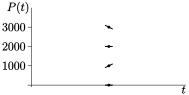
\includegraphics{pop1}
\end{center}
\end{efig}
As a result,
\begin{itemize}
  \item  if $P(0)=0$, the graph starts out horizontally. In other
    words, as $t$ starts to increase, $P(t)$ remains at zero, so the slope
    of the graph remains at zero. The population
    size remains zero for all time. As a check, observe that
    the function $P(t)=0$ obeys $\diff{P}{t}(t)=\big(6000-3P(t)\big)P(t)$
    for all $t$.

  \item  Similarly, if $P(0)=2000$, the graph again starts out
    horizontally. So $P(t)$ remains at $2000$ and the slope remains at zero.
    The population size remains 2000 for all time. Again, the function
    $P(t)=2000$ obeys $\diff{P}{t}(t)=\big(6000-3P(t)\big)P(t)$ for all $t$.

  \item  If $P(0)=1000$, the graph starts out with positive slope.
    So $P(t)$ increases with $t$. As $P(t)$ increases towards 2000, the slope
    $(6000-3P(t)\big)P(t)$, while remaining positive, gets closer and closer
    to zero. As the graph approaches height 2000, it becomes more and more
    horizontal. The graph cannot actually cross from below 2000 to above 2000,
    because to do so it would have to have strictly positive slope for
    some value of $P$ above 2000, which is not allowed.
%\issue{Joel:\\Mention\\uniqueness\\of solutions\\to IVP's?}

  \item  If $P(0)=3000$, the graph starts out with negative slope.
    So $P(t)$ decreases with $t$. As $P(t)$ decreases towards 2000, the slope
    $(6000-3P(t)\big)P(t)$, while remaining negative, gets closer and closer
    to zero. As the graph approaches height 2000, it becomes more and more
    horizontal. The graph cannot actually cross from above 2000 to below 2000,
    because to do so it would have to have negative slope for some value of
    $P$ below 2000, which is not allowed.
\end{itemize}

\noindent These curves are sketched in the figure below. We conclude that
for any initial population size $P(0)$, except $P(0)=0$, the population
size approaches $2000$ as $t\rightarrow\infty$.

\begin{efig}
\begin{center}
   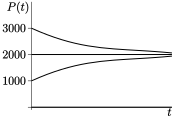
\includegraphics{pop2}
\end{center}
\end{efig}

\noindent Now we'll do an example in which we explicitly solve the logistic
growth equation.

\begin{eg}\label{eg:SDElogisticA}
 In 1986, the population of the world was 5 billion and was
increasing at a rate of 2\% per year. Using the logistic growth model
with an assumed maximum population of 100 billion, predict the population
of the world in the years 2000, 2100 and 2500.


\soln Let $y(t)$ be the population of the world, in billions of people,
at time $1986+t$. The logistic growth model assumes
\begin{equation*}
y'=ay(K-y)
\end{equation*}
where $K$ is the carrying capacity and $a=\frac{b_0}{K}$.

First we'll determine the values of the constants $a$ and $K$ from the
given data.
\begin{itemize}\itemsep1pt \parskip0pt \parsep0pt %\itemindent-15pt
\item
We know  that, if at time zero the population is below $K$, then as time
increases the population increases, approaching the limit $K$ as $t$ tends
to infinity. So in this problem $K$ is the maximum population. That is,
$K=100$.
\item
 We are also told that, at time zero, the percentage rate of change
of population, $100\frac{y'}{y}$, is 2, so that, at time zero,
$\frac{y'}{y}=0.02$.
But, from the differential equation, $\frac{y'}{y}=a(K-y)$. Hence at time
zero, $0.02=a(100-5)$, so that $a= \frac{2}{9500}$.
\end{itemize}
We now know $a$ and $K$ and can solve the (separable) differential equation
\begin{align*}
\frac{\dee{y}}{dt}=ay(K-y)&\implies
\frac{\dee{y}}{y(K-y)}=a\,\dee{t}\implies
\int\frac{1}{K}\Big[\frac{1}{y}-\frac{1}{y-K}\Big]\dee{y}=\int a\,\dee{t}\\
&\implies \frac{1}{K}[\log |y|-\log|y-K|]=at+C \\
&\implies  \log\frac{|y|}{|y-K|}=aKt+CK\implies
\Big|\frac{y}{y-K}\Big|=De^{aKt}
\end{align*}
with $D=e^{CK}$. We know that $y$ remains between $0$ and $K$, so that
$\Big|\frac{y}{y-K}\Big|=\frac{y}{K-y}$ and our solution obeys
\begin{equation*}
\frac{y}{K-y}=De^{aKt}
\end{equation*}
At this stage, we know the values of the constants $a$ and $K$, but not
the value of the constant $D$.
We are given that at $t=0$, $y=5$. Subbing in this, and the values of $K$
and $a$,
\begin{equation*}
\frac{5}{100-5}=De^{0}
\implies D=\frac{5}{95}
\end{equation*}
So the solution obeys the algebraic equation
\begin{equation*}
 \frac{y}{100-y}=\frac{5}{95}e^{2t/95}
\end{equation*}
which we can solve to get $y$ as a function of $t$.
\begin{align*}
 y=(100-y)\frac{5}{95}e^{2t/95}
     &\implies 95y=(500-5y)e^{2t/95} \\
     &\implies \big(95+5e^{2t/95}\big)y=500 e^{2t/95} \\
     &\implies y=\frac{500e^{2t/95}}{95+5e^{2t/95}}
=\frac{100e^{2t/95}}{19+e^{2t/95}}
=\frac{100}{1+19e^{-2t/95}}
\end{align*}
Finally,
\begin{itemize}\itemsep1pt \parskip0pt \parsep0pt %\itemindent-15pt
\item  In the year 2000, $t=14$ and
                 $y=\frac{100}{1+19e^{-28/95}}\approx6.6$ billion.
\item  In the year 2100, $t=114$ and
                $y=\frac{100}{1+19e^{-228/95}}\approx 36.7$ billion.
\item  In the year 2200, $t=514$ and
                $y=\frac{100}{1+19e^{-1028/95}}\approx 100$ billion.
\end{itemize}
\end{eg}



%%%%%%%%%%%%%%%%%%%%%%%%%%%%%%%%%%%%%%%%%%%%%%%%%%%%%%%%%%%%%%%%%
\subsection{Optional --- Mixing Problems}
%%%%%%%%%%%%%%%%%%%%%%%%%%%%%%%%%%%%%%%%%%%%%%%%%%%%%%%%%%%%%%%%%

\begin{eg}\label{eg:SDEmixingA}
At time $t=0$, where $t$ is measured in minutes, a tank with
a 5--litre capacity contains 3 litres of water in which 1 kg of salt
is dissolved. Fresh water enters the tank at a rate of 2 litres per
minute and the fully mixed solution leaks out of the tank at the
\emph{varying} rate of $2t$ litres per minute.
\begin{enumerate}[(a)]
\item Determine the volume of solution $V(t)$ in the tank at time
$t$.
\item Determine the amount of salt $Q(t)$ in solution when the
amount of water in the tank is at maximum.
\end{enumerate}

\soln (a) The rate of change of the volume in the tank, at time $t$,
is $2-2t$, because water is entering at a rate $2$ and solution is
leaking out at a rate $2t$. Thus
\begin{equation*}
\diff{V}{t}=2-2t
\implies \dee{V}=(2-2t)\,\dee{t}
\implies V=\int (2-2t)\,\dee{t}
=2t-t^2+C
\end{equation*}
at least until $V(t)$ reaches either the capacity of the tank or zero.
When $t=0$, $V=3$ so $C=3$ and $V(t)=3+2t-t^2$. Observe that
$V(t)$ is at a maximum when $\diff{V}{t}=2-2t=0$, or $t=1$.

\medskip
\noindent (b) In the very short time interval from time $t$ to time $t+\dee{t}$,
 $2t\,\dee{t}$ litres of brine leaves the tank. That is, the fraction
$\frac{2t\,\dee{t}}{V(t)}$ of the total salt in the tank,
namely $Q(t)\frac{2t\,\dee{t}}{V(t)}$ kilograms, leaves. Thus salt is leaving the
tank at the rate
\begin{equation*}
\frac{Q(t)\frac{2t\,\dee{t}}{V(t)}}{\dee{t}}
=\frac{2tQ(t)}{V(t)}
=\frac{2tQ(t)}{3+2t-t^2} \text{ kilograms per minute}
\end{equation*}
so
\begin{align*}
\diff{Q}{t}=-\frac{2tQ(t)}{3+2t-t^2}
&\implies
\frac{dQ}{Q}=-\frac{2t}{3+2t-t^2}\dee{t}=-\frac{2t}{(3-t)(1+t)}\dee{t}
=\Big[\frac{3/2}{t-3}+\frac{1/2}{t+1}\Big]\dee{t}\\
&\implies
\log Q=\frac{3}{2}\log|t-3|+\frac{1}{2}\log|t+1|+C
\end{align*}
We are interested in the time interval $0\le t\le 1$. In this time interval
$|t-3|=3-t$ and $|t+1|=t+1$ so
\begin{equation*}
\log Q=\frac{3}{2}\log(3-t)+\frac{1}{2}\log(t+1)+C
\end{equation*}
At $t=0$, $Q$ is 1 so
\begin{equation*}
\log 1=\frac{3}{2}\log(3-0)+\frac{1}{2}\log(0+1)+C
\implies
C=\log 1-\frac{3}{2}\log 3-\frac{1}{2}\log 1=-\frac{3}{2}\log 3
\end{equation*}
At $t=1$
\begin{equation*}
\log Q=\frac{3}{2}\log(3-1)+\frac{1}{2}\log(1+1)-\frac{3}{2}\log 3
=2\log 2-\frac{3}{2}\log 3
=\log 4 -\log 3^{\nicefrac{3}{2}}
\end{equation*}
so $Q=\frac{4}{3^{\nicefrac{3}{2}}}$.
\end{eg}
\goodbreak

\begin{eg}\label{eg:SDEmixingB}
A tank contains 1500 liters of brine with a concentration of $0.3$ kg of
salt per liter. Another brine solution, this with a concentration of
$0.1$ kg of salt per liter is poured into the tank at a rate of $20$ li/min.
At the same time, $20$ li/min of the solution in the tank, which is stirred
continuously, is drained from the tank.
\begin{enumerate}[(a)]
\item How many kilograms of salt will remain in the tank after
half an hour?
\item How long will it take to reduce the concentration to $0.2$
kg/li?
\end{enumerate}

\soln
Denote by $Q(t)$ the amount of salt in the tank at time $t$.
In a very short time interval $\dee{t}$, the incoming solution adds $20\, \dee{t}$
liters of a solution carrying $0.1$ kg/li. So the incoming solution adds
$0.1\times 20\, \dee{t}=2\, \dee{t}$ kg of salt. In the same time interval
$20\, \dee{t}$ liters is drained from the tank. The concentration of the
drained brine is $\frac{Q(t)}{1500}$. So $\frac{Q(t)}{1500} 20\, \dee{t}$ kg were
removed. All together, the change in the salt content of the tank during
the short time interval is
\begin{equation*}
dQ=2\, \dee{t}-\frac{Q(t)}{1500} 20\, \dee{t}
=\Big(2-\frac{Q(t)}{75}\Big) \dee{t}
\end{equation*}
The rate of change of salt content per unit time is
\begin{equation*}
\frac{dQ}{dt}=2-\frac{Q(t)}{75}
=-\frac{1}{75}\big(Q(t)-150\big)
\end{equation*}
The solution of this equation  is
\begin{equation*}
Q(t)=\big\{Q(0)-150\big\}e^{-t/75} + 150
\end{equation*}
by Theorem \ref{thm:linearODE}, with $a=-\frac{1}{75}$ and $b=150$.
At time $0$, $Q(0)=1500\times 0.3=450$. So
\begin{equation*}
Q(t)=150+300e^{-t/75}
\end{equation*}

\noindent (a) At $t=30$
\begin{equation*}
Q(30)=150+300e^{-30/75}=\text{351.1 kg}
\end{equation*}

\noindent (b) $Q(t)=0.2\times 1500=300$ kg is achieved when
\begin{align*}
&150+300e^{-t/75}=300\implies 300e^{-t/75}=150
\implies e^{-t/75}=0.5\cr
&\implies -\frac{t}{75}=\log (0.5)
\implies t=-75\log (0.5)=\text{51.99 min}
\end{align*}
\end{eg}

%%%%%%%%%%%%%%%%%%%%%%%%%%%%%%%%%%%%%%%%%%%%%%%%%%%%%%%%%%%%%%%%%
\subsection{Optional --- Interest on Investments}
%%%%%%%%%%%%%%%%%%%%%%%%%%%%%%%%%%%%%%%%%%%%%%%%%%%%%%%%%%%%%%%%%


Suppose that you deposit $\$P$ in a bank account at time $t=0$.
The account pays $r\%$ interest per year compounded $n$ times per year.

\begin{itemize} \itemsep1pt \parskip0pt
  \item  The first interest payment is made at time $t=\frac{1}{n}$.
         Because the balance in the account during the time interval
         $0<t<\frac{1}{n}$ is $\$P$ and interest is being paid for
         $\big(\frac{1}{n}\big)^{\rm th}$ of a year, that first
         interest payment is $\frac{1}{n}\times\frac{r}{100}\times P$.
         After the first interest payment, the balance in the account is
         $P+\frac{1}{n}\times\frac{r}{100}\times P
          =  \big(1+\frac{r}{100n}\big)P$.
  \item  The second interest payment is made at time $t=\frac{2}{n}$.
         Because the balance in the account during the time interval
         $\frac{1}{n}<t<\frac{2}{n}$ is $\big(1+\frac{r}{100n}\big)P$
         and interest is being paid for $\big(\frac{1}{n}\big)^{\rm th}$
         of a year, the second  interest payment is
          $\frac{1}{n}\times\frac{r}{100}\times \big(1+\frac{r}{100n}\big)P$.
         After the second interest payment, the balance in the account is
         $\big(1+\frac{r}{100n}\big)P+\frac{1}{n}\times\frac{r}{100}\times
         \big(1+\frac{r}{100n}\big)P
          =  \big(1+\frac{r}{100n}\big)^2P$.
  \item  And so on.
\end{itemize}
In general, at time $t=\frac{m}{n}$ (just after the $m^{\rm th}$ interest
payment),
the balance in the account is
\begin{equation}\label{eq:SDEdiscreteCompounding}
         B(t) = \Big(1+\frac{r}{100n}\Big)^m P
              = \Big(1+\frac{r}{100n}\Big)^{nt}P
\end{equation}
Three common values of $n$ are $1$ (interest is paid once a year),
$12$ (i.e. interest is paid once a month) and 365 (i.e. interest
is paid daily). The limit $n\rightarrow\infty$ is called continuous
compounding\footnote{There are banks that advertise continuous compounding.
You can find some by googling ``interest is compounded continuously and
paid''}. Under continuous compounding, the balance at time $t$ is
\begin{align*}
B(t) &= \lim_{n\rightarrow\infty} \Big(1+\frac{r}{100n}\Big)^{nt}P
\end{align*}
You may have already seen the limit
\begin{equation}\label{eq:SDEexpLimit}
\lim_{x\rightarrow 0}(1+x)^{a/x}=e^a
\end{equation}
If so, you can evaluate $B(t)$ by applying \eqref{eq:SDEexpLimit}
with $x=\frac{r}{100n}$ and $a=\frac{rt}{100}$ (so that $\frac{a}{x}=nt$).
As $n\rightarrow \infty$, $x\rightarrow 0$ so that
\begin{equation}\label{eq:SDEcontinuousCompounding}
B(t) = \lim_{n\rightarrow\infty} \Big(1+\frac{r}{100n}\Big)^{nt}P
     =\lim_{x\rightarrow 0}(1+x)^{a/x}P=e^aP
     = e^{rt/100}P
\end{equation}
If you haven't seen \eqref{eq:SDEexpLimit} before, that's OK.
In the following example, we rederive \eqref{eq:SDEcontinuousCompounding}
using a differential equation instead of \eqref{eq:SDEexpLimit}.
%%%%%%%%%%%%%%%%%%%%%%%%%
\begin{eg}\label{eg:SDEmoneyA}
Suppose, again, that you deposit $\$P$ in a bank
account at time $t=0$, and that the account pays $r\%$ interest per year
compounded $n$ times per year, and denote by $B(t)$ the balance at time
$t$. Suppose that you have just received an interest payment at time $t$.
Then the next interest payment will be made at time $t+\frac{1}{n}$
and will be $\frac{1}{n}\times\frac{r}{100}\times B(t)=\frac{r}{100n}B(t)$.
So, calling $\frac{1}{n}=h$,
\begin{equation*}
B(t+h)=B(t) + \frac{r}{100}B(t)h\qquad\text{or}\qquad
\frac{B(t+h)-B(t)}{h} = \frac{r}{100}B(t)
\end{equation*}
To get continuous compounding we take the limit $n\rightarrow\infty$
or, equivalently, $h\rightarrow 0$. This gives
\begin{equation*}
\lim_{h\rightarrow 0}\frac{B(t+h)-B(t)}{h} = \frac{r}{100}B(t)
\qquad\text{or}\qquad
\diff{B}{t}(t) = \frac{r}{100}B(t)
\end{equation*}
By Theorem \ref{thm:linearODE}, with $a=\frac{r}{100}$ and $b=0$,
(or Corollary \ref{cor:carbonDating} with $k=-\frac{r}{100}$),
\begin{align*}
B(t)=e^{rt/100}B(0)=e^{rt/100}P
\end{align*}
once again.
\end{eg}
\goodbreak
%%%%%%%%%%%%%%%%%%%%%%%%%
\begin{eg}\label{eg:SDEmoneyB}
\begin{enumerate}[(a)]
\item A bank advertises that it compounds interest continuously and that
it will double your money in ten years. What is the annual interest rate?

\item A bank advertises that it compounds monthly and that it will
double your money in ten years. What is the annual interest rate?
\end{enumerate}

\soln (a)
Let the interest rate be $r\%$ per year. If you start with $\$P$, then
after $t$ years, you have $Pe^{rt/100}$, under continuous compounding.
This was \eqref{eq:SDEcontinuousCompounding}.
After 10 years you have $Pe^{r/10}$. This is supposed to be $2P$, so
$$
Pe^{r/10}=2P\quad\Longrightarrow\quad
e^{r/10}=2\quad\Longrightarrow\quad
\frac{r}{10}=\log 2\quad\Longrightarrow\quad
r=10\log2 =6.93\%
$$

\noindent (b)
Let the interest rate be $r\%$ per year. If you start with $\$P$, then
after $t$ years, you have $P\big(1+\frac{r}{100\times 12}\big)^{12 t}$,
under monthly compounding. This was \eqref{eq:SDEdiscreteCompounding}.
After 10 years you have $P\big(1+\frac{r}{100\times 12}\big)^{120}$. This is
supposed to be $2P$, so
\begin{align*}
&P\big(1+\frac{r}{100\times 12}\big)^{120}=2P
&&\Longrightarrow\quad
    \big(1+\frac{r}{1200}\big)^{120}=2\quad\Longrightarrow\quad
1+\frac{r}{1200}=2^{1/120}\\
&\Longrightarrow\quad \frac{r}{1200}=2^{1/120}-1
&&\Longrightarrow\quad
r=1200\big(2^{1/120}-1\big) =6.95\%
\end{align*}
\end{eg}

%%%%%%%%%%%%%%%%%%%%%%%%%
\begin{eg}\label{eg:SDEmoneyC}
A 25 year old graduate of UBC is given \$50,000 which is invested
at 5\% per year compounded continuously. The graduate also intends to
deposit money continuously at the rate of \$2000 per year.
\begin{enumerate}[(a)]
\item  Find a differential equation that $A(t)$ obeys, assuming that
the interest rate remains 5\%.

\item  Determine the amount of money in the account when the graduate
is 65.

\item  At age 65, the graduate will start withdrawing money
continuously at the rate of $W$ dollars per year. If the money
must last until the person is 85, what is the largest possible
value of $W$?
\end{enumerate}

\soln (a) Let's consider what happens to $A$ over a very short time
interval from time $t$ to time $t + \De t$. At time $t$ the account balance
is $A(t)$. During the (really short) specified time interval the balance
remains very close to $A(t)$ and so earns interest of
$\frac{5}{100}\times\De t\times A(t)$.  During the same time interval,
the graduate also deposits an additional $\$ 2000\De t$. So
\begin{equation*}
A(t+\De t)\approx A(t) + 0.05 A(t)\De t+ 2000\De t
\implies
\frac{A(t+\De t)- A(t)}{\De t} \approx 0.05 A(t)  + 2000
\end{equation*}
In the limit $\De t\rightarrow 0$, the approximation becomes exact and
we get
\begin{equation*}
\diff{A}{t}= 0.05 A+2000
\end{equation*}

\noindent (b) The amount of money at time $t$ obeys
\begin{equation*}
\diff{A}{t}= 0.05 A(t)+2,\!000=0.05\big(A(t)+40,\!000\big)
\end{equation*}
So by Theorem \ref{thm:linearODE}
(with $a=0.05$ and $b=-40,\!000$),
\begin{equation*}
A(t)=\big(A(0)+40,\!000\big)e^{0.05 t} -40,\!000
\end{equation*}
At time 0 (when the graduate is 25), $A(0)=50,\!000$, so the amount of
money at time $t$ is
\begin{equation*}
A(t)=90,\!000\, e^{0.05 t}-40,000
\end{equation*}
In particular, when the graduate is 65 years old, $t=40$ and
\begin{equation*}
A(40)=90,\!000\, e^{0.05 \times 40}-40,000=\text{\$625,015.05 }
\end{equation*}

\noindent(c) When the graduate stops depositing money and instead
starts withdrawing money at a rate $W$, the equation for $A$ becomes
\begin{equation*}
\diff{A}{t}= 0.05 A-W= 0.05 (A-20 W)
\end{equation*}
assuming that the interest rate remains 5\%.
This time, Theorem \ref{thm:linearODE} (with $a=0.05$ and $b=20W$) gives
\begin{equation*}
A(t)=\big(A(0)-20W\big)e^{0.05 t} + 20W
\end{equation*}
If we now reset our clock so that $t=0$ when the graduate is 65,
$A(0)=625,015.05$. So the amount of money at time $t$ is
\begin{equation*}
A(t)=20W+ e^{0.05 t}(625,015.05-20W)
\end{equation*}
We want the account to be depleted when the graduate is 85. So, we
want $A(20)=0$. This is the case if
\begin{align*}
20W+ e^{0.05\times 20}(625,015.05-20W)=0
&\implies
20W+ e(625,015.05-20W)=0\\
&\implies
20(e-1)W= 625,015.05e\\
&\implies
W=\frac{625,015.05e}{20(e-1)}=\$49,437.96
\end{align*}
\end{eg}




\begin{comment}
\section{(Optional) --- more about numerical integration}
%%%%%%%%%%%%%%%%%%%%%%%%%%%%%%%%%%%%%%%%%%%%%%%%%%%%%%%%%
\subsection*{Richardson Extrapolation\footnote{Richardson extrapolation
was introduced by the Englishman Lewis Fry Richardson
(1881--1953) in 1911.} (Optional)}
%%%%%%%%%%%%%%%%%%%%%%%%%%%%%%%%%%%%%%%%%%%%%%%%%%%%%%%%%
%\issue{Joel:\\ Eliminate?\\ Optional?}
There are many approximation procedures in which one first picks a
step size $h$ and then generates an approximation $A(h)$ to some
desired quantity $A$. Often the order of the error generated by the
procedure is known. This means
\begin{equation}\label{eq:ErrorOrderFull}
A=A(h)+Kh^k+K'h^{k+1}+K''h^{k+2}+\ \cdots
\end{equation}
with $k$ being some known constant, called the order of the error, and $K,\ K',\ K'',\
\cdots$ being some other
(usually unknown) constants. For example, $A$ might be the value of
some integral $\int_a^b f(x)\,\dee{x}$. For the trapezoidal rule with $n$ steps,
$\De x=\tfrac{b-a}{n}$ plays the
role of the step size. If $A(h)$ is the approximation to $A$ produced
by trapezoidal rule with $\De x=h$, then $k=2$. If Simpson's rule
is used, $k=4$.

Let's first suppose that $h$ is small enough that the terms
$K'h^{k+1}+K''h^{k+2}+\ \cdots$ in \eqref{eq:ErrorOrderFull} are small
enough that dropping them has essentially no impact.
This would give
\begin{equation}\label{eq:ErrorOrderSimple}
A=A(h)+Kh^k
\end{equation}
Imagine that we know $k$, but that we do not know $A$ or $K$,
and think of \eqref{eq:ErrorOrderSimple} as an equation that
the unknowns $A$ and $K$ have to solve. It may look like have
one equation in the two unknowns $K$, $A$, but that is \emph{not}
the case.
The reason is that \eqref{eq:ErrorOrderSimple} is (essentially) true for
all (sufficiently small) choices of $h$.
If we pick some $h$, say $h_1$, and use the algorithm to determine $A(h_1)$
then \eqref{eq:ErrorOrderSimple}, with $h$ replaced by $h_1$, gives
one equation in the two unknowns $A$ and $K$, and if we then
pick some
different $h$, say $h_2$, and use the algorithm a second time
to determine $A(h_2)$
then \eqref{eq:ErrorOrderSimple}, with $h$ replaced by $h_2$, gives a
second equation in the two unknowns $A$ and $K$. The two equations will
then determine both $A$ and $K$.

To be concrete, suppose that we have picked some specific value of $h$, and
have chosen $h_1=h$ and $h_2=\tfrac{h}{2}$, and that we have evaluated
$A(h)$ and $A(h/2)$. Then the two equations are
\begin{subequations}\label{eq:RichardDerive}
\begin{align}
A&=A(h)+Kh^k \\
A&=A\big(\tfrac{h}{2}\big)+K\big(\tfrac{h}{2}\big)^k
\end{align}
\end{subequations}
It is now easy to solve for both $K$ and $A$. To get $K$ just subtract
(\ref{eq:RichardDerive}b) from (\ref{eq:RichardDerive}a).
\begin{subequations}\label{eq:RichardApprox}
\begin{equation}
(\ref{eq:RichardDerive}\textrm{a})-(\ref{eq:RichardDerive}\textrm{b}):\quad
0=A(h)-A\big(\tfrac{h}{2}\big) +\big(1-\tfrac{1}{2^k}\big)Kh^k
\quad\implies\quad
K=\frac{A(\nicefrac{h}{2})-A(h)}{[1-2^{-k}]h^k}
\end{equation}
To get $A$ multiply (\ref{eq:RichardDerive}b) by $2^k$ and then
subtract (\ref{eq:RichardDerive}a).
\begin{equation}
2^k(\ref{eq:RichardDerive}\textrm{b})-(\ref{eq:RichardDerive}\textrm{a}):\quad
[2^k-1]A=2^kA\big(\tfrac{h}{2}\big)-A(h)
\quad\implies\quad
A=\frac{2^kA(\nicefrac{h}{2})-A(h)}{2^k-1}
\end{equation}
\end{subequations}
The generation of a ``new improved'' approximation
for $A$ from two $A(h)$'s with different values of $h$ is called Richardson
Extrapolation.

\begin{eg}\label{eg:Richard}
Applying the trapezoidal rule to the integral $\int_0^1\frac{4}{1+x^2}\dee{x}$
with step sizes $\frac{1}{8}$ and $\frac{1}{16}$
(i.e. with $n=8$ and $n=16$) gives, with $h=\frac{1}{8}$,
\begin{equation*}
A(h)=3.1389884945\qquad
A\big(\tfrac{h}{2}\big)=3.1409416120
\end{equation*}
So (\ref{eq:RichardApprox}\textrm{b}), with $k=2$, gives us
the ``new improved'' approximation
\begin{equation*}
\frac{2^2\times 3.1409416120 -3.1389884945}{2^2-1}=3.1415926512
\end{equation*}
This new approximation really is ``improved'':
\begin{itemize}\itemsep1pt \parskip0pt \parsep0pt %\itemindent-15pt
\item $A\big(\tfrac{1}{8}\big)$ agrees with $\pi$ to two decimal places,
\item $A\big(\tfrac{1}{16}\big)$  agrees with $\pi$ to three decimal places
            and
\item the new approximation  agrees with $\pi$ to eight decimal places.
\end{itemize}
% The real $\pi=3.141592653589793$
Beware that (\ref{eq:RichardDerive}b) is saying that $K\big(\nicefrac{h}{2}\big)^k$ is
(approximately)
the error in $A\big(\nicefrac{h}{2}\big)$, not the error in $A$. You cannot
get an ``even more improved'' approximation by using
(\ref{eq:RichardApprox}\textrm{a}) to compute $K$ and then adding
$K\big(\nicefrac{h}{2}\big)^k$ to the ``new improved''
approximation (\ref{eq:RichardApprox}\textrm{b}).
\end{eg}

\begin{eg}[Example \ref{eg:SimpsonErr} revisited]\label{eg:SimpsonErrB}
Suppose again that  we wish to use Simpson's rule to evaluate
$\int_0^1 e^{-x^2}\,\dee{x}$ to within an accuracy of $10^{-6}$, but that we
do not need the degree of certainty provided by Example \ref{eg:SimpsonErr}.
A commonly used strategy is to
\begin{itemize}
\item first apply Simpson's rule twice with some relatively small number
of steps and
\item then use (\ref{eq:RichardApprox}a), with $k=4$, to determine $K$ and
\item then use the condition $|K| h^k\le 10^{-6}$ to determine, approximately,
the number of steps required
\item and finally apply Simpson's rule with the number of steps just determined.
\end{itemize}
Let's implement this strategy. First we apply Simpson's rule with step sizes
$\tfrac{1}{4}$ and $\tfrac{1}{8}$. Writing $\tfrac{1}{4}=h'$, we get
\begin{equation*}
A(h')=0.74685538  % 0.746855379790987
\qquad
A(h'/2)=0.74682612 %0.746826120527467
\end{equation*}
so that (\ref{eq:RichardApprox}a), with $k=4$ and $h$ replaced
by $h'$, yields
\begin{equation*}
K=\frac{0.74682612 - 0.74685538}{[1-2^{-4}](1/4)^4}
%=-\frac{0.000031211}{(1/4)^4}
=-7.990\times 10^{-3}
\end{equation*}
We want to use a step size $h$ obeying
\[
|K|h^4\le 10^{-6}
\iff 7.990\times 10^{-3} h^4\le 10^{-6}
\iff h \le\root{4}\of{\frac{1}{7990}} =\frac{1}{9.45}
\]
like, for example, $h=\tfrac{1}{10}$. Applying Simpson's rule with
$h=\tfrac{1}{10}$ gives
\begin{equation*}
A\big(\tfrac{1}{10}\big) = 0.74682495
\end{equation*}
The exact answer, to eight decimal places, is $0.74682413$ so the error
in $A\big(\tfrac{1}{10}\big)$ is indeed just under $10^{-6}$.
\end{eg}


%%%%%%%%%%%%%%%%%%%%%%%%%%%%%%%%%%%%%%%%%%%%%%%%%%%%%%%%%
\subsection*{Romberg Integration\footnote{Romberg Integration
was introduced by the German Werner Romberg (1909--2003) in
1955.}}
%%%%%%%%%%%%%%%%%%%%%%%%%%%%%%%%%%%%%%%%%%%%%%%%%%%%%%%%%

The formulae (\ref{eq:RichardApprox}\textrm{a,b}) for $K$ and $A$ are,
of course, only approximate since
they are based on \eqref{eq:ErrorOrderSimple}, which is an approximation
to \eqref{eq:ErrorOrderFull}. Let's repeat the derivation that leads to
\eqref{eq:RichardApprox}, but using the full \eqref{eq:ErrorOrderFull},
\begin{equation*}
A=A(h)+Kh^k+K'h^{k+1}+\cdots
\end{equation*}
Once again, suppose that we have chosen some $h$ and that we have
evaluated $A(h)$ and $A(h/2)$. They obey
\begin{subequations}\label{eq:RichardDeriveFull}
\begin{align}
A&=A(h)+Kh^k+K'h^{k+1}+\cdots \\
A&=A\big(\tfrac{h}{2}\big)+K\big(\tfrac{h}{2}\big)^k
        +K'\big(\tfrac{h}{2}\big)^{k+1}+\cdots
\end{align}
\end{subequations}
Now, as we did in the derivation of (\ref{eq:RichardApprox}\textrm{b}) , multiply
(\ref{eq:RichardDeriveFull}b) by $2^k$ and then
subtract (\ref{eq:RichardDeriveFull}a). This gives
\begin{equation*}
\left(2^k-1\right)A=2^kA(h/2)-A(h)-\half K' h^{k+1}+\cdots
\end{equation*}
and then, dividing across by $\left(2^k-1\right)$,
\begin{equation*}
A=\frac{2^kA(h/2)-A(h)}{2^k-1}-\frac{1/2}{2^k-1} K' h^{k+1}+\cdots
\end{equation*}
Hence if we define our ``new improved approximation''
\begin{equation}\label{eq:RichardsonB}
B(h)=\frac{2^kA(h/2)-A(h)}{2^k-1}\qquad\text{and}\qquad
\tilde K = -\frac{1/2}{2^k-1}K'
\end{equation}
we have
\begin{equation*}%\label{eq:RichardsonAB}
A=B(h)+\tilde K h^{k+1}+\cdots
\end{equation*}
which says that $B(h)$ is an approximation to $A$ whose error is of order $k+1$,
one better than $A(h)$'s.

If $A(h)$ has been computed for three values of $h$, we can generate $B(h)$
for two values of $h$ and repeat the above procedure with a new value of
$k$. And so on.
One widely used numerical integration algorithm,
called Romberg integration, applies this procedure repeatedly to the
trapezoidal rule. It is known that the trapezoidal rule approximation
$T(h)$ to an integral $I$ has error behaviour (assuming that the integrand
$f(x)$ is smooth)
\begin{equation*}
I=T(h)+K_1h^2+K_2h^4+K_3h^6+\cdots
\end{equation*}
Only even powers of $h$ appear.
Hence
\begin{align*}
T(h)&                         &&\hbox{ has error of order 2, so that,
using \eqref{eq:RichardsonB} with $k=2$,}\\
T_1(h)&=\tfrac{4T(h/2)-T(h)}{3}&&\hbox{ has error of order 4, so that,
using \eqref{eq:RichardsonB} with $k=4$,}\\
T_2(h)&=\tfrac{16T_1(h/2)-T_1(h)}{15}&&\hbox{ has error of order 6, so that,
using \eqref{eq:RichardsonB} with $k=6$,}\\
T_3(h)&=\tfrac{64T_2(h/2)-T_2(h)}{63}&&\hbox{ has error of order 8 and so on}
\end{align*}
We know another method which produces an error of order 4 --- Simpson's
rule. In fact, $T_1(h)$ is exactly Simpson's rule (for step size
$\tfrac{h}{2}$).

\begin{eg}\label{eg:Romberg3}
The following table\footnote{The second column, for example,
of the table only reports $5$ decimal places for $T(h)$.
But many more decimal places of $T(h)$ were used in the computations
of $T_1(h)$ etc.}
illustrates Romberg integration by applying it to
the area $A$ of the integral $A=\int_0^1\frac{4}{1+x^2}\dee{x}$.
The exact value of this integral is $\pi$ which is $3.14159265358979$,
to fourteen decimal places.


\begin{center}
     \begin{tabular}{|c|c|c|c|c|}
          \hline
          $h$ & $T(h)$ & $T_1(h)$ & $T_2(h)$ & $T_3(h)$\\ \hline
      1/4 & 3.13118
          & 3.14159250246
          & 3.14159266114
          & 3.14159265359003
          \\ \hline
      1/8 & 3.13899
          & 3.141592651225
          & 3.141592653708
          \\ \cline{1-4}
     1/16 & 3.14094
          & 3.141592653553
          \\ \cline{1-3}
     1/32 & 3.14143
     \\ \cline{1-2}
     \end{tabular}
\end{center}
This computation required the evaluation of $f(x)=\frac{4}{1+x^2}$ only
for $x=\nicefrac{n}{32}$ with $0\le n\le 32$ --- that is, a total
of $33$ evaluations of $f$. Those $33$ evaluations gave us $12$
correct decimal places. By way of comparison, $T\big(\nicefrac{1}{32}\big)$
used the same $33$ evaluations of $f$, but only gave us $3$ correct
decimal places.
\end{eg}


\intremark{
\begin{eg}\label{eg:Romberg}
The following table illustrates Romberg integration by applying it to
the integral $A=\int_0^\pi\sin x\ \dee{x}=2$.


\begin{center}
     \begin{tabular}{|c|c|c|c|c|}
          \hline
          $h$ & $T(h)$ & $T_1(h)$ & $T_2(h)$ & $T_3(h)$  \\
          \hline
       $\pi/4$ & 1.896
               & 2.0002692
               & 1.999999752
               & 2.000000000060 \\ \hline
      $\pi/$8 & 1.974
              & 2.0000166
              & 1.999999996 \\ \cline{1-4}
      $\pi/16$ & 1.993
              & 2.0000010  \\ \cline{1-3}
      $\pi/32$ & 1.998  \\ \cline{1-2}
     \end{tabular}
\end{center}

\noindent The next table gives the percentage error for each of the
entries in the above table.

\renewcommand{\arraystretch}{1.3}
\begin{center}
     \begin{tabular}{|c|c|c|c|c|}
          \hline
          $h$ & $100\tfrac{2-T(h)}{2}$
              & $100\tfrac{2-T_1(h)}{2}$
              & $100\tfrac{2-T_2(h)}{2}$
              & $100\tfrac{2-T_3(h)}{2}$  \\
          \hline
       $\pi/4$ &  5.2
               & $-1.3\times 10^{-2}$
               & $1.2\times 10^{-5}$
               & $-2.9\times 10^{-9}$ \\ \hline
      $\pi/$8 & 1.3
              & $-8.3\times 10^{-4}$
              & $1.9\times 10^{-7}$ \\ \cline{1-4}
      $\pi/16$ &0.32
              & $-5.2\times 10^{-5}$ \\ \cline{1-3}
      $\pi/32$ & 0.08 \\ \cline{1-2}
     \end{tabular}
\end{center}
\renewcommand{\arraystretch}{1.0}
\end{eg}

\begin{eg}\label{eg:Romberg2}
The following table illustrates Romberg integration by applying it to
the integral $A=\int_0^1\tfrac{\dee{x}}{1+x^2}$. The exact value of this integral
is $\tfrac{\pi}{4}$ which is $0.78539816339745$, to fourteen decimal places.


\begin{center}
     \begin{tabular}{|c|c|c|c|c|}
          \hline
          $h$ & $T(h)$ & $T_1(h)$ & $T_2(h)$ & $T_3(h)$\\ \hline
      1/4 & 0.78279
          & 0.785398125615
          & 0.785398165285
          & 0.78539816339751 \\ \hline
      1/8 & 0.78475
          & 0.785398162806
          & 0.785398163427 \\ \cline{1-4}
     1/16 & 0.78524
          & 0.785398163388 \\ \cline{1-3}
     1/32 & 0.78536 \\ \cline{1-2}
     \end{tabular}
\end{center}
This computation required the evaluation of $f(x)=\frac{1}{1+x^2}$ only
for $x=\nicefrac{n}{32}$ with $0\le n\le 32$.
\end{eg}
}

%%%%%%%%%%%%%%%%%%%%%%%%%%%%%%%%%%%%%%%%%%%%%%%%%%%%%%%%%
\subsection*{Optional --- Adaptive Quadrature}
%%%%%%%%%%%%%%%%%%%%%%%%%%%%%%%%%%%%%%%%%%%%%%%%%%%%%%%%%
%\issue{Joel: \\ Eliminate?}
Richardson extrapolation is also used to choose the step size
so as to achieve some desired degree of accuracy. ``Adaptive quadrature''
refers to a family of algorithms that use small step sizes
in the part of the domain of integration where it is hard to get good
accuracy and large step sizes in the part of the domain of integration
where it is easy to get good accuracy.

We'll illustrate the idea using Simpson's rule applied to the
integral $\int_a^b f(x)\ \dee{x}$, and assuming that we want the error
to be no more than (approximately) $\veps$. Denote by $S(a',b'\,;\,h')$,
the answer given when Simpson's rule is applied to the integral
$\int_{a'}^{b'} f(x)\ \dee{x}$ with step size $h'$.
\begin{itemize}
\item \emph{Step 1.} We start by applying Simpson's rule, combined
with Richardson extrapolation so as to get an error estimate,
with the largest step size $h$ that we can. Set $h=\tfrac{b-a}{2}$
and compute
\[
f(a)\quad
f\big(a+\tfrac{h}{2}\big)\quad
f(a+h)=f\big(\tfrac{a+b}{2}\big)\quad
f\big(a+\tfrac{3h}{2}\big)\quad
f(a+2h)=f(b)
\]
Then
\[
S\big(a,b\,;h\big)
=\tfrac{h}{3}\big\{f(a)+4 f\big(a+h\big)+f(b)\big\}\quad\text{and}\quad
S\big(a,b\,;\tfrac{h}{2}\big)
=S\big(a,\tfrac{a+b}{2}\,;\tfrac{h}{2}\big)
+S\big(\tfrac{a+b}{2},b\,;\tfrac{h}{2}\big)
\]
with
\begin{align*}
S\big(a,\tfrac{a+b}{2}\,;\,\tfrac{h}{2}\big)
&=\tfrac{h}{6}\big\{f(a)+4 f\big(a+\tfrac{h}{2}\big)
           +f\big(\tfrac{a+b}{2}\big)\big\} \\
S\big(\tfrac{a+b}{2},b\,;\,\tfrac{h}{2}\big)
&=\tfrac{h}{6}\big\{f\big(\tfrac{a+b}{2}\big)+4 f\big(a+\tfrac{3h}{2}\big)
           +f(b)\big\}
\end{align*}
Using the Richardson extrapolation formula (\ref{eq:RichardApprox}a)
with $k=4$ gives that the error in $S\big(a,b\,;\,\tfrac{h}{2}\big)$
is (approximately)
\begin{equation}\label{eq:adaptiveEg}
\big|K\big(\tfrac{h}{2}\big)^4\big|=\tfrac{1}{15}\Big|
             S\big(a,b\,;\,\tfrac{h}{2}\big)
            -S\big(a,b\,;\,h\big)\Big|
\end{equation}
If this is smaller than $\veps$, we have (approximately) the desired
accuracy and stop. (It is very common to build in a bit of a safety
margin and require that, for example, $\big|K\big(\tfrac{h}{2}\big)^4\big|$
be smaller than $\tfrac{\veps}{2}$ rather than $\veps$.)
%%%%
\item \emph{Step 2.} If \eqref{eq:adaptiveEg} is larger than $\veps$,
we divide the original integral $I=\int_a^b f(x)\,\dee{x}$ into two ``half--sized''
integrals, $I_1=\int_a^{\tfrac{a+b}{2}} f(x)\,\dee{x}$ and
 $I_2=\int_{\tfrac{a+b}{2}}^b f(x)\,\dee{x}$ and repeat the procedure of Step 1
on each of them, but with $h$ replaced by $\tfrac{h}{2}$ and
$\veps$ replaced by $\tfrac{\veps}{2}$ --- if we can find an approximation,
$\tilde I_1$, to $I_1$ with an error less than $\tfrac{\veps}{2}$ and an
approximation, $\tilde I_2$, to $I_2$ with an error less than
$\tfrac{\veps}{2}$, then $\tilde I_1+\tilde I_2$
approximates $I$ with an error less than $\veps$.
%%%%
\item \emph{Steps 3, 4, 5, $\cdots$} Repeat as required.
\end{itemize}

\begin{eg}\label{eg:adaptiveQuad}
Let's apply adaptive quadrature using Simpson's rule as above with the
goal of computing $\int _0^1\sqrt{x}\ \dee{x}$ with an error of at most
$\veps=0.0005=5\times 10^{-4}$.
\begin{itemize}
\item \emph{Step 1 -- the interval $[0,1]$.} (The notation $[0,1]$ stands
for the interval $0\le x\le 1$.)
\begin{align*}
S(0,1\,;\half)&= 0.63807119 \\
S(0,\half\,;\tfrac{1}{4})&= 0.22559223 \\
S(\half,1\,;\tfrac{1}{4})&= 0.43093403  \\
\text{error}&=\tfrac{1}{15}\Big|S(0,\half\,;\tfrac{1}{4})
                              +S(\half,1\,;\tfrac{1}{4})
                              -S(0,1\,;\half)\Big|
             =0.0012 >\veps =0.0005
\end{align*}
This is unacceptably large, so we subdivide the interval $[0,1]$ into
the two halves $\big[0,\tfrac{1}{2}\big]$ and
$\big[\tfrac{1}{2},1\big]$ and apply
the procedure separately to each half.

\item \emph{Step 2a -- the interval $[0,\half]$.}
\begin{align*}
S(0,\half\,;\tfrac{1}{4})&= 0.22559223 \\
S(0,\tfrac{1}{4}\,;\tfrac{1}{8})&= 0.07975890 \\
S(\tfrac{1}{4},\half\,;\tfrac{1}{8})&= 0.15235819 \\
\text{error}&=\tfrac{1}{15}\Big|S(0,\tfrac{1}{4}\,;\tfrac{1}{8})
                              +S(\tfrac{1}{4},\half\,;\tfrac{1}{8})
                              -S(0,\half\,;\tfrac{1}{4})\Big|
             = 0.00043  >\tfrac{\veps}{2} = 0.00025
\end{align*}


\item \emph{Step 2b -- the interval $[\half,1]$.}
\begin{align*}
S(\half,1\,;\tfrac{1}{4})&= 0.43093403 \\
S(\half,\tfrac{3}{4}\,;\tfrac{1}{8})&= 0.19730874 \\
S(\tfrac{3}{4},1\,;\tfrac{1}{8})&= 0.23365345  \\
\text{error}&=\tfrac{1}{15}\Big|S(\half,\tfrac{3}{4}\,;\tfrac{1}{8})
                              +S(\tfrac{3}{4},1\,;\tfrac{1}{8})
                              -S(\half,1\,;\tfrac{1}{4})\Big|
             = 0.0000019 <\tfrac{\veps}{2} = 0.00025
\end{align*}

\item\emph{Step 2 resum\'e.} The error for the interval $[0,\half]$ is
unacceptably large, so we subdivide the interval $[0,\half]$ into
the two halves $[0,\tfrac{1}{4}]$ and $[\tfrac{1}{4},\half]$
and apply the procedure separately to each half. The error for the interval
$[\half,1]$ is small enough, so we accept
\[
S(\half,1\,;\tfrac{1}{8})
  = S(\half,\tfrac{3}{4}\,;\tfrac{1}{8})
   + S(\tfrac{3}{4},1\,;\tfrac{1}{8})
  = 0.43096219
\]
as the approximate value of $\int_{1/2}^1\sqrt{x}\,\dee{x}$.

\item \emph{Step 3a -- the interval $[0,\tfrac{1}{4}]$.}
\begin{align*}
S(0,\tfrac{1}{4}\,;\tfrac{1}{8})&= 0.07975890  \\
S(0,\tfrac{1}{8}\,;\tfrac{1}{16})&= 0.02819903   \\
S(\tfrac{1}{8},\tfrac{1}{4}\,;\tfrac{1}{16})&= 0.05386675   \\
\text{error}&=\tfrac{1}{15}\Big|S(0,\tfrac{1}{8}\,;\tfrac{1}{16})
                              +S(\tfrac{1}{8},\tfrac{1}{4}\,;\tfrac{1}{16})
                              -S(0,\tfrac{1}{4}\,;\tfrac{1}{8})\Big|
             = 0.000153792 > \tfrac{\veps}{4} = 0.000125
\end{align*}


\item \emph{Step 3b -- the interval $[\tfrac{1}{4},\tfrac{1}{2}]$.}
\begin{align*}
S(\tfrac{1}{4},\half\,;\tfrac{1}{8})&= 0.15235819   \\
S(\tfrac{1}{4},\tfrac{3}{8}\,;\tfrac{1}{16})&= 0.06975918  \\
S(\tfrac{3}{8},\half\,;\tfrac{1}{16})&= 0.08260897   \\
\text{error}&=\tfrac{1}{15}\Big|S(\tfrac{1}{4},\tfrac{3}{8}\,;\tfrac{1}{16})
                              +S(\tfrac{3}{8},\half\,;\tfrac{1}{16})
                              -S(\tfrac{1}{4},\half\,;\tfrac{1}{8})\Big|
             =  0.00000066  <\tfrac{\veps}{4} = 0.000125
\end{align*}

\item\emph{Step 3 resum\'e.} The error for the interval $[0,\tfrac{1}{4}]$ is
unacceptably large, so we subdivide the interval $[0,\tfrac{1}{4}]$ into
the two halves $[0,\tfrac{1}{8}]$ and $[\tfrac{1}{8},\tfrac{1}{4}]$
and apply the procedure separately to each half. The error for the interval
$[\tfrac{1}{4},\half]$ is small enough, so we accept
\[
S(\tfrac{1}{4},\half\,;\tfrac{1}{16})
  = S(\tfrac{1}{4},\tfrac{3}{8}\,;\tfrac{1}{16})
   + S(\tfrac{3}{8},\half\,;\tfrac{1}{16})
  = 0.15236814
\]
as the approximate value of $\int_{1/4}^{1/2}\sqrt{x}\,\dee{x}$.

\item \emph{Step 4a -- the interval $[0,\tfrac{1}{8}]$.}
\begin{align*}
S(0,\tfrac{1}{8}\,;\tfrac{1}{16})&= 0.02819903   \\
S(0,\tfrac{1}{16}\,;\tfrac{1}{32})&= 0.00996986    \\
S(\tfrac{1}{16},\tfrac{1}{8}\,;\tfrac{1}{32})&= 0.01904477    \\
\text{error}&=\tfrac{1}{15}\Big|S(0,\tfrac{1}{16}\,;\tfrac{1}{32})
                              +S(\tfrac{1}{16},\tfrac{1}{8}\,;\tfrac{1}{32})
                              -S(0,\tfrac{1}{8}\,;\tfrac{1}{16})\Big|
             =  0.000054  < \tfrac{\veps}{8} = 0.0000625
\end{align*}


\item \emph{Step 4b -- the interval $[\tfrac{1}{8},\tfrac{1}{4}]$.}
\begin{align*}
S(\tfrac{1}{8},\tfrac{1}{4}\,;\tfrac{1}{16})&= 0.05386675   \\
S(\tfrac{1}{8},\tfrac{3}{16}\,;\tfrac{1}{32})&= 0.02466359  \\
S(\tfrac{3}{16},\tfrac{1}{4}\,;\tfrac{1}{32})&= 0.02920668   \\
\text{error}&=\tfrac{1}{15}\Big|S(\tfrac{1}{8},\tfrac{3}{16}\,;\tfrac{1}{32})
                              +S(\tfrac{3}{6},\tfrac{1}{4}\,;\tfrac{1}{32})
                              -S(\tfrac{1}{8},\tfrac{1}{4}\,;\tfrac{1}{16})\Big|
             =  0.00000024  <\tfrac{\veps}{8} = 0.0000625
\end{align*}


\item\emph{Step 4 resum\'e.} The error for the interval
$[0,\tfrac{1}{8}]$ is small enough, so we accept
\[
S(0,\tfrac{1}{8}\,;\tfrac{1}{32})
  = S(0,\tfrac{1}{16}\,;\tfrac{1}{32})
   + S(\tfrac{1}{16},\tfrac{1}{8}\,;\tfrac{1}{32})
  =  0.02901464
\]
as the approximate value of $\int_0^{1/8}\sqrt{x}\,\dee{x}$.
The error for the interval
$[\tfrac{1}{8},\tfrac{1}{4}]$ is small enough, so we accept
\[
S(\tfrac{1}{8},\tfrac{1}{4}\,;\tfrac{1}{32})
  = S(\tfrac{1}{8},\tfrac{3}{16}\,;\tfrac{1}{32})
   + S(\tfrac{3}{16},\tfrac{1}{4}\,;\tfrac{1}{32})
  = 0.05387027
\]
as the approximate value of $\int_{1/8}^{1/4}\sqrt{x}\,\dee{x}$.

\item\emph{Conclusion} The approximate value for $\int_0^1\sqrt{x}\ \dee{x}$
is
\[
S(0,\tfrac{1}{8}\,;\tfrac{1}{32})
+S(\tfrac{1}{8},\tfrac{1}{4}\,;\tfrac{1}{32})
+S(\tfrac{1}{4},\half\,;\tfrac{1}{16})
+S(\half,1\,;\tfrac{1}{8})
=0.66621525
\]
Of course the exact value of $\int_0^1\sqrt{x}\ \dee{x}=\tfrac{2}{3}$,
so the actual error in our approximation is
\[
\tfrac{2}{3}-0.66621525 = 0.00045 <\veps = 0.0005
\]


\end{itemize}

\end{eg}
%%%%%%%%%%%%%%%%%%%%%%%%%
\intremark{%%%%%%%%%%  INTERNAL RMARK - more decimal places
\noindent More decimal places

\begin{itemize}
\item \emph{Step 1 -- the interval $[0,1]$.}
\begin{align*}
S(0,1\,;\half)&= 0.638071187457698 \\
S(0,\half\,;\tfrac{1}{4})&= 0.225592231765546 \\
S(\half,1\,;\tfrac{1}{4})&= 0.430934033027025 \\
\text{error}&=\tfrac{1}{15}\Big|S(0,\half\,;\tfrac{1}{4})
                              +S(\half,1\,;\tfrac{1}{4})
                              -S(0,1\,;\half)\Big|
             =0.001230338>\veps =0.0005
\end{align*}
This is unacceptably large, so we subdivide the interval $[0,1]$ into
the two halves $\big[0,\tfrac{1}{2}\big]$ and
$\big[\tfrac{1}{2},1\big]$ and apply
the procedure separately to each half.

\item \emph{Step 2a -- the interval $[0,\half]$.}
\begin{align*}
S(0,\half\,;\tfrac{1}{4})&= 0.225592231765546 \\
S(0,\tfrac{1}{4}\,;\tfrac{1}{8})&= 0.079758898432212 \\
S(\tfrac{1}{4},\half\,;\tfrac{1}{8})&= 0.152358188498739 \\
\text{error}&=\tfrac{1}{15}\Big|S(0,\tfrac{1}{4}\,;\tfrac{1}{8})
                              +S(\tfrac{1}{4},\half\,;\tfrac{1}{8})
                              -S(0,\half\,;\tfrac{1}{4})\Big|
             = 0.00043499  >\tfrac{\veps}{2} = 0.00025
\end{align*}


\item \emph{Step 2b -- the interval $[\half,1]$.}
\begin{align*}
S(\half,1\,;\tfrac{1}{4})&= 0.430934033027025 \\
S(\half,\tfrac{3}{4}\,;\tfrac{1}{8})&= 0.197308743547474 \\
S(\tfrac{3}{4},1\,;\tfrac{1}{8})&= 0.233653449606599  \\
\text{error}&=\tfrac{1}{15}\Big|S(\half,\tfrac{3}{4}\,;\tfrac{1}{8})
                              +S(\tfrac{3}{4},1\,;\tfrac{1}{8})
                              -S(\half,1\,;\tfrac{1}{4})\Big|
             = 0.000001877 <\tfrac{\veps}{2} = 0.00025
\end{align*}

\item\emph{Step 2 resum\'e.} The error for the interval $[0,\half]$ is
unacceptably large, so we subdivide the interval $[0,\half]$ into
the two halves $[0,\tfrac{1}{4}]$ and $[\tfrac{1}{4},\half]$
and apply the procedure separately to each half. The error for the interval
$[\half,1]$ is small enough, so we accept
\[
S(\half,1\,;\tfrac{1}{8})
  = S(\half,\tfrac{3}{4}\,;\tfrac{1}{8})
   + S(\tfrac{3}{4},1\,;\tfrac{1}{8})
  = 0.430962193
\]
as the approximate value of $\int_{1/2}^1\sqrt{x}\,\dee{x}$.


\item \emph{Step 3a -- the interval $[0,\tfrac{1}{4}]$.}
\begin{align*}
S(0,\tfrac{1}{4}\,;\tfrac{1}{8})&= 0.079758898432212  \\
S(0,\tfrac{1}{8}\,;\tfrac{1}{16})&= 0.028199028970693  \\
S(\tfrac{1}{8},\tfrac{1}{4}\,;\tfrac{1}{16})&= 0.053866754128378  \\
\text{error}&=\tfrac{1}{15}\Big|S(0,\tfrac{1}{8}\,;\tfrac{1}{16})
                              +S(\tfrac{1}{8},\tfrac{1}{4}\,;\tfrac{1}{16})
                              -S(0,\tfrac{1}{4}\,;\tfrac{1}{8})\Big|
             = 0.000153792 > \tfrac{\veps}{4} = 0.000125
\end{align*}


\item \emph{Step 3b -- the interval $[\tfrac{1}{4},\tfrac{1}{2}]$.}
\begin{align*}
S(\tfrac{1}{4},\half\,;\tfrac{1}{8})&= 0.152358188498739  \\
S(\tfrac{1}{4},\tfrac{3}{8}\,;\tfrac{1}{16})&= 0.069759175274908  \\
S(\tfrac{3}{8},\half\,;\tfrac{1}{16})&= 0.082608969332228  \\
\text{error}&=\tfrac{1}{15}\Big|S(\tfrac{1}{4},\tfrac{3}{8}\,;\tfrac{1}{16})
                              +S(\tfrac{3}{8},\half\,;\tfrac{1}{16})
                              -S(\tfrac{1}{4},\half\,;\tfrac{1}{8})\Big|
             =  0.000000664  <\tfrac{\veps}{4} = 0.000125
\end{align*}

\item\emph{Step 3 resum\'e.} The error for the interval $[0,\tfrac{1}{4}]$ is
unacceptably large, so we subdivide the interval $[0,\tfrac{1}{4}]$ into
the two halves $[0,\tfrac{1}{8}]$ and $[\tfrac{1}{8},\tfrac{1}{4}]$
and apply the procedure separately to each half. The error for the interval
$[\tfrac{1}{4},\half]$ is small enough, so we accept
\[
S(\tfrac{1}{4},\half\,;\tfrac{1}{16})
  = S(\tfrac{1}{4},\tfrac{3}{8}\,;\tfrac{1}{16})
   + S(\tfrac{3}{8},\half\,;\tfrac{1}{16})
  = 0.152368145
\]
as the approximate value of $\int_{1/4}^{1/2}\sqrt{x}\,\dee{x}$.

\item \emph{Step 4a -- the interval $[0,\tfrac{1}{8}]$.}
\begin{align*}
S(0,\tfrac{1}{8}\,;\tfrac{1}{16})&= 0.028199028970693   \\
S(0,\tfrac{1}{16}\,;\tfrac{1}{32})&= 0.009969862304027   \\
S(\tfrac{1}{16},\tfrac{1}{8}\,;\tfrac{1}{32})&= 0.019044773562342   \\
\text{error}&=\tfrac{1}{15}\Big|S(0,\tfrac{1}{16}\,;\tfrac{1}{32})
                              +S(\tfrac{1}{16},\tfrac{1}{8}\,;\tfrac{1}{32})
                              -S(0,\tfrac{1}{8}\,;\tfrac{1}{16})\Big|
             =  0.000054374 < \tfrac{\veps}{8} = 0.0000625
\end{align*}


\item \emph{Step 4b -- the interval $[\tfrac{1}{8},\tfrac{1}{4}]$.}
\begin{align*}
S(\tfrac{1}{8},\tfrac{1}{4}\,;\tfrac{1}{16})&= 0.053866754128378   \\
S(\tfrac{1}{8},\tfrac{3}{16}\,;\tfrac{1}{32})&= 0.024663592943434  \\
S(\tfrac{3}{16},\tfrac{1}{4}\,;\tfrac{1}{32})&= 0.029206681200825  \\
\text{error}&=\tfrac{1}{15}\Big|S(\tfrac{1}{8},\tfrac{3}{16}\,;\tfrac{1}{32})
                              +S(\tfrac{3}{6},\tfrac{1}{4}\,;\tfrac{1}{32})
                              -S(\tfrac{1}{8},\tfrac{1}{4}\,;\tfrac{1}{16})\Big|
             =  0.000000235  <\tfrac{\veps}{8} = 0.0000625
\end{align*}


\item\emph{Step 4 resum\'e.} The error for the interval
$[0,\tfrac{1}{8}]$ is small enough, so we accept
\[
S(0,\tfrac{1}{8}\,;\tfrac{1}{32})
  = S(0,\tfrac{1}{16}\,;\tfrac{1}{32})
   + S(\tfrac{1}{16},\tfrac{1}{8}\,;\tfrac{1}{32})
  =  0.029014636
\]
as the approximate value of $\int_0^{1/8}\sqrt{x}\,\dee{x}$.
The error for the interval
$[\tfrac{1}{8},\tfrac{1}{4}]$ is small enough, so we accept
\[
S(\tfrac{1}{8},\tfrac{1}{4}\,;\tfrac{1}{32})
  = S(\tfrac{1}{8},\tfrac{3}{16}\,;\tfrac{1}{32})
   + S(\tfrac{3}{16},\tfrac{1}{4}\,;\tfrac{1}{32})
  = 0.053870274
\]
as the approximate value of $\int_{1/8}^{1/4}\sqrt{x}\,\dee{x}$.

\item\emph{Conclusion} The approximate value for $\int_0^1\sqrt{x}\ \dee{x}$
is
\[
S(0,\tfrac{1}{8}\,;\tfrac{1}{32})
+S(\tfrac{1}{8},\tfrac{1}{4}\,;\tfrac{1}{32})
+S(\tfrac{1}{4},\half\,;\tfrac{1}{16})
+S(\half,1\,;\tfrac{1}{8})
=0.666215248
\]
Of course the exact value of $\int_0^1\sqrt{x}\ \dee{x}=\tfrac{2}{3}$,
so the actual error in our approximation is
\[
\tfrac{2}{3}-0.666215248 = 0.000451419 <\veps = 0.0005
\]


\end{itemize}
}%%%%%%%%%%%%%%%%%%%   END INTERNAL REMARK - more decimal places
\end{comment}
